%% Copernicus Publications Manuscript Preparation Template for LaTeX Submissions
\documentclass[gmd, manuscript]{copernicus} %final manuscript

\begin{document}
\title{GGCMI Phase II: globally gridded crop simulation model response to uniform changes in CO$_2$, temperature, water, and nitrogen levels}

\Author[1,2]{James}{Franke}
\Author[2,3]{Joshua}{Elliott}
\Author[4]{Christoph}{M\"{u}ller}
\Author[5]{Alexander}{Ruane}
\Author[6]{Abigail}{Snyder}
\Author[3,2,4,5]{Jonas}{J\"{a}germeyr}
\Author[7,8]{Juraj}{Balkovic}
\Author[9,10]{Philippe}{Ciais}
\Author[11]{Marie}{Dury}
\Author[12]{Pete}{Falloon}
\Author[7]{Christian}{Folberth}
\Author[11]{Louis}{Fran{\c{c}}ois}
\Author[13]{Tobias}{Hank}
\Author[14,23]{Munir}{Hoffmann}
\Author[15,16]{R.\ Cesar}{Izaurralde}
\Author[11]{Ingrid}{Jacquemin}
\Author[15]{Curtis}{Jones}
\Author[7]{Nikolay}{Khabarov}
\Author[14]{Marian}{Koch}
\Author[2,17]{Michelle}{Li}
\Author[9,18]{Wenfeng}{Liu}
\Author[19]{Stefan}{Olin}
\Author[5,20]{Meridel}{Phillips}
\Author[21,22]{Thomas A.\ M.}{Pugh}
\Author[15]{Ashwan}{Reddy}
\Author[9,10]{Xuhui}{Wang}
\Author[12]{Karina}{Williams}
\Author[13]{Florian}{Zabel}
\Author[1,2]{Elisabeth}{Moyer}
%%%%%%%%%%%%%%%%%%%%%%%%%%%%%%
\affil[1]{Department of the Geophysical Sciences, University of Chicago, Chicago, IL, USA}
\affil[2]{Center for Robust Decision-making on Climate and Energy Policy (RDCEP), University of Chicago, Chicago, IL, USA}
\affil[3]{Department of Computer Science, University of Chicago, Chicago, IL, USA}
\affil[4]{Potsdam Institute for Climate Impact Research, Leibniz Association (Member), Potsdam, Germany}
\affil[5]{NASA Goddard Institute for Space Studies, New York, NY, United States}
\affil[6]{Joint Global Change Research Institute, Pacific Northwest National Laboratory, College Park, MD, USA}
\affil[7]{Ecosystem Services and Management Program, International Institute for Applied Systems Analysis, Laxenburg, Austria}
\affil[8]{Department of Soil Science, Faculty of Natural Sciences, Comenius University in Bratislava, Bratislava, Slovak Republic}
\affil[9]{Laboratoire des Sciences du Climat et de l'Environnement, CEA-CNRS-UVSQ, 91191 Gif-sur-Yvette, France}
\affil[10]{Sino-French Institute of Earth System Sciences, College of Urban and Env. Sciences, Peking University, Beijing, China}
\affil[11]{Unit{\'{e}} de Mod{\'{e}}lisation du Climat et des Cycles Biog\'eochimiques, UR SPHERES, Institut d'Astrophysique et de G\'eophysique, University of Li\`ege, Belgium}
\affil[12]{Met Office Hadley Centre, Exeter, United Kingdom}
\affil[13]{Department of Geography, Ludwig-Maximilians-Universit\"{a}t, Munich, Germany}
\affil[14]{Georg-August-University G\"{o}ttingen, Tropical Plant Production and Agricultural Systems Modelling, G\"{o}ttingen, Germany}
\affil[15]{Department of Geographical Sciences, University of Maryland, College Park, MD, USA}
\affil[16]{Texas Agrilife Research and Extension, Texas A\&M University, Temple, TX, USA}
\affil[17]{Department of Statistics, University of Chicago, Chicago, IL, USA}
\affil[18]{EAWAG, Swiss Federal Institute of Aquatic Science and Technology, D\"{u}bendorf, Switzerland}
\affil[19]{Department of Physical Geography and Ecosystem Science, Lund University, Lund, Sweden}
\affil[20]{Earth Institute Center for Climate Systems Research, Columbia University, New York, NY, USA}
\affil[21]{School of Geography, Earth and Environmental Sciences, University of Birmingham, Birmingham, UK.}
\affil[22]{Birmingham Institute of Forest Research, University of Birmingham, Birmingham, UK.}
\affil[23]{Leibniz Centre for Agricultural Landscape Research (ZALF), D-15374 Müncheberg, Germany}
%%%%%%%%%%%%%%%%%%%%%%%%%%%%%%
\runningtitle{The GGCMI Phase II experiment: simulating and emulating global crop yield}
\runningauthor{Franke et al.}
\correspondence{James Franke (jfranke@uchicago.edu)}
%%%%%%%%%%%%%%%%%%%%%%%%%%%%%%
%% These dates will be inserted by Copernicus Publications during the typesetting process.
\received{}
\pubdiscuss{} %% only important for two-stage journals
\revised{}
\accepted{}
\published{}
%%%%%%%%%%%%%%%%%%%%%%%%%%%%%%
\firstpage{1}
\maketitle
%%%%%%%%%%%%%%%%%%%%%%%%%%%%%%
\begin{abstract}
Concerns about food security under climate change motivate efforts to better understand future changes in crop yields.  
Process-based crop models, which represent plant physiological processes, are necessary tools for this purpose since they allow representing future conditions not sampled in the historical record and new locations where cultivation may shift. 
However, models remain uncertain and differ in many critical details. 
The Global Gridded Crop Model Intercomparison (GGCMI) Phase II experiment, an activity of the Agricultural Model Intercomparison and Improvement Project (AgMIP), is designed to allow systematic evaluation and ``emulation'' of model responses to multiple interacting factors, including carbon dioxide, temperature, water availability, and nitrogen application (CTWN). 
In this paper we describe the GGCMI Phase II experimental protocol (simulations run with systematic uniform perturbations of historical climate) and its simulations (from twelve crop models and five crops); identify responses that are robust across models and those that remain uncertain; and present an emulator or statistical representation of model responses. 
Modeled yields show robust decreases to warmer mean climatologies in almost all regions, with a nonlinear dependence that means yield changes in warmer baseline locations are more sensitive to temperature increases. 
Inter-model uncertainty is qualitatively similar across all the four input dimensions, but is highest in high-latitude regions where crops may be grown in the future.
\end{abstract}

%\copyrightstatement{TEXT}

\introduction
\label{S:1}
Understanding crop yield response to a changing climate is critically important, especially as the global food production system will face pressure from increased demand over the next century \citep{bodirsky2015}. 
Climate-related reductions in supply could therefore have severe socioeconomic consequences \citep[e.g.][]{Stevanovic2016,Wiebe_2015}. 
Multiple studies using different crop or climate models concur in projecting sharp yield reductions on currently cultivated cropland under {business-as-usual} climate scenarios, although their yield projections show considerable spread \citep[e.g.][and references therein]{Rosenzweig2014, Schauberger2017, porter2014}. 
Modeling crop responses continues to be challenging, as crop growth is a function of complex interactions between climate inputs and management practices \citep{Boote13,rotter2011}. 
Intercomparison projects such as the Agricultural Model Intercomparison and Improvement Project \citep[AgMIP][]{ROSENZWEIG2013} have helped to quantify uncertainties in model projections \citep{Rosenzweig2014}, developed protocols \citep{Elliott2015} for evaluating model performance \citep{muller_global_2017} and analyzed selected mechanisms \citep[e.g.][]{Schauberger2017}. 

% to me, this is too broad of an introduction and the distinction of different modle types is more suitable for pitching the emulators than for the introduction of the experiment

%Computational models have been used to project crop yields since the 1950's, beginning with statistical models  that attempt to capture the relationship between input factors and resultant yields \citep[e.g.][]{Heady57, Heady61}. 
%These statistical models were typically developed on a small scale for locations with extensive histories of yield data. 
%The emergence of electronic computers allowed development of numerical models that simulate the process of photosynthesis and the biology and phenology of individual crops (first proposed by \citet{wit58} and \citet{Duncan67} and attempted by \citet{Duncan72}; for a history of crop model development see \citet{Rosenzweig2014}). 
%A half-century of improvement in both models and computing resources means that researchers can now run crop simulations for many years at higher spatial resolution on the global scale. 

%Both types of models continue to be used, and comparative studies have concluded that when done carefully, both approaches can provide similar yield estimates \citep[e.g.][]{Lobell2010, Moore2017, Roberts2017, zhao2017}. 
Models tend to agree broadly in major response patterns, including a reasonable representation of the spatial pattern in historical yields of major crops \citep[e.g.][]{Elliott2015, muller_global_2017} and projections of shifts in yield under future climate scenarios.

Process-based models still struggle with some important details, including reproducing historical year-to-year variability in various countries \citep[e.g.][]{muller_global_2017}, reproducing historical yields when driven by reanalysis weather \citep[e.g.][]{Glotter14}, and low sensitivity to extreme events \citep[e.g.][]{Glotter15, Jag2018, schewe2019}. 
These issues are driven in part by the diversity of new cultivars and genetic variants, which outstrips the ability of academic modeling groups to capture them \citep[e.g.][]{JONES2017b}. 
Models also do not simulate many additional factors affecting production, including but not limited to: pests, diseases, and weeds. 
For these reasons, individual studies must generally re-calibrate models to ensure that short-term predictions reflect current cultivars and management levels, and long-term projections retain considerable uncertainty \citep{WOLF2002217, JAGTAP200273, Iizumi2010, ANGULO201332, Asseng2013, Asseng2015}. 
Inter-model discrepancies can also be high in areas not yet cultivated \citep[e.g.][]{Challinor2014, WHITE2011357}. 
Finally, process-based models present additional difficulties for high-resolution global studies because of their complexity and computational requirements, as well as the general inability to calibrate site-specific parameters. 
%For global economic impacts assessments, it is often impossible to integrate a set of process-based crop models directly into an integrated assessment model to estimate the potential cost of climate change to the agricultural sector.

Nevertheless, process-based models are necessary for understanding the future yield impacts of climate change as well as options for climate mitigation \citep{muller2015} and adaptation \citep{challinor2018improving}, future sustainable development \citep{humpenoder2018large}, and food security \citep{wheeler2013climate}. 
Despite the additional uncertainty and challenges to run crop models at the global scale \citep{muller_global_2017}, gridded, global crop model applications are much needed for consistent assessments.
Climate change and international agricultural trade often require to consider the global and local dynamics \citep{rosenzweig2018,ruane2018} and global market mechanisms may strongly modulate climate change impacts \citep{Stevanovic2016,hasegawa2018risk}.
Cultivation may shift to new areas, where no yield data are currently available and therefore statistical models cannot be applied. 
%Yield data, on which statistical models could be trained, are also often limited in the developing world, where future climate impacts may be the most critical. 
Finally, only process-based models can capture the growth response to novel conditions and practices that are not represented in historical data \citep[e.g.][]{pugh_climate_2016, Roberts2017}. 
These novel changes can include the direct fertilization effect of elevated CO$_2$, and changes in management practices that may mitigate climate-induced damages \citep[e.g.][]{minoli2019modelling}.

Understanding process-based models' responses to important drivers are thus critical to improve future projections of agricultural productivity.
The Global Gridded Crop Model Intercomparison (GGCMI) of AgMIP \citep{Elliott2015} has thus designed a 2nd phase (\textit{Phase II}) with a focus on models' response to changes in the most important model drivers: atmospheric carbon dioxide concentrations ([CO$_2$], C),temperature (T), water (W), and nitrogen (N). 
The CTWN experiment is inspired by AgMIP's Coordinated Climate-Crop Modeling Project \citep[C3MP][]{ruane2014,mcdermid2015agmip} and has been extended by the nitrogen dimension. 
To account for the importance of adapation in agricultural production to climate change, a fifth dimension, adaptation (A) has been added to the CTWN experiment. 
The {A} dimension only has two elements, namely \textit{no adaptation} and one \textit{adapation} setting, in which the growing season that is shortened under warming, is regained by adapted crop cultivar choice.

The Global Gridded Crop Model Intercomparison (GGCMI) Phase II experiment was conducted by a suite of process-based crop models, running across historical conditions perturbed by a set of discrete steps in the four input parameters (CTWN), for both adaptation settings (yes/no). 
The experimental protocol involves 756 different parameter combinations for each model and crop for the non-adapted and 648 combinations for the adapted setting (does not include T=0), with simulations providing near-global coverage at a half degree spatial resolution. 
The experiment was conducted as part of the Agricultural Model Intercomparison and Improvement Project (AgMIP) \citep{ROSENZWEIG2013, Rosenzweig2014}, an international effort conducted under a framework similar to the Climate Model Intercomparison Project (CMIP) \citep{Taylor2012, Eyring2016}. 
The GGCMI protocol builds on the AgMIP Coordinated Climate-Crop Modeling Project (C3MP) \citep{ruane2014, mcdermid2015agmip} and contributes to the AgMIP Coordinated Global and Regional Assessments (CGRA) \citep{ruane2018, rosenzweig2018}. 
GGCMI Phase II is designed to allow addressing goals such as understanding where highest-yield regions may shift under climate change; exploring future adaptive management strategies; understanding how interacting input drivers affect crop yield; quantifying uncertainties across models and major drivers; and testing strategies for producing lightweight emulators of process-based models. 
In this paper, we describe the GGCMI Phase II model experiments and present initial summary results.


%%%%%%%%%%%%%%%%%%%%%%%%%%%%%%%%%%%%%%%%%%%%%%%%%%%%%%%%%%%%%%%
%%%%%%%%%%%%%%%%%%%%%%%%%%%%%%%%%%%%%%%%%%%%%%%%%%%%%%%%%%%%%%%
%%%%%%%%%%%%%%%%%%%%%%%%%%%%%%%%%%%%%%%%%%%%%%%%%%%%%%%%%%%%%%%
\section{Methods}
\label{S:2}

\subsection{Modeling protocol}

GGCMI Phase II is the continuation of a multi-model comparison exercise begun in 2014. 
The initial Phase I compared harmonized yield simulations of 21 models for 19 crops over the historical period with a primary goal of model evaluation \citep{Elliott2015, muller_global_2017} and understanding of different sources of uncertainty, such as model parameterization \citep{folberth2016}, different weather products, or aggregation \citep{porwollik_spatial_2016}. 
Phase II compares simulations of 12 models for 5 crops (maize, rice, soybean, spring wheat, and winter wheat) using only one of the weather products used in Phase I, which was then perturbed systematically for the different simulations. 
The reduced set of crops includes the three major global cereals and the major legume and accounts for over 50\% of human calories (in 2016, nearly 3.5 billion tons or 32\% of total global crop production by weight \citep{FAOSTAT}, which were also in the focus of analyses in the previous analyses \citep{Elliott2015,muller_global_2017,porwollik_spatial_2016} and for which global sub-national reference data exist \citep{Ray2012,iizumi_historical_2014}. 

The guiding scientific rationale of GGCMI Phase II is to provide a comprehensive, systematic evaluation of the response of process-based crop models to [CO$_2$], temperature, water, and applied nitrogen (collectively referred to as ``CTWN''). Given that the production of annual crops is continuously changing by making use of new varieties and technologies \citep{olesen2012changes} it is plausible to assume at least some degree of adaptation to new climate conditions. We thus also include one additional simulation set across the entire CTWN space with just one simple adaptation setting (A), in which we assume that varieties are grown at each temperature level, that maintain the growing season, i.e. that reach maturity at the same time as current varieties under current temperature regimes. We acknowledge that this is an overly simplistic assumption that does not reflect the range of opportunities and limitations to adaptation \citep{vadez2012adaptation,challinor2018improving}. Still, this setting allows to demonstrate the role of adaptation and is easy to integrate into the modeling protocol as growing seasons have to be harmonized across groups anyway.
The dataset is designed to allow researchers to:
\begin{itemize}
    \item Enhance understanding of how models work by characterizing their sensitivity to input climate and nitrogen drivers.
    \item Study the interactions between climate variables and nitrogen inputs in driving modeled yield impacts. 
    \item Explore differences in crop response to warming across the Earth's climate regions.
    \item Provide a dataset that allows statistical emulation of crop model responses for downstream modelers.
    \item Illustrate differences in potential adaptation via growing season changes. 
\end{itemize}
\vspace{-0.05in}

The experimental protocol consists of 9 levels for precipitation perturbations, 7 for temperature, 4 for [CO$_2$], and 3 for applied nitrogen, for a total of 672 simulations for rainfed agriculture and an additional 84 for irrigated (Table \ref{table:inputs}). 
For irrigated simulations, limitations from actual water supply are not considered. 
Limits for the climate variable perturbations are selected to represent reasonable ranges for potential climate changes in the medium term. 
Note that [CO$_2$] changes are applied independently of changes in climate variables, so that higher [CO$_2$] is not associated with higher temperatures. 
The resulting GGCMI Phase II dataset captures a distribution of crop responses over the potential space of future climate conditions.

Each model is run at 0.5 degree spatial resolution and covers all currently cultivated areas and much of the uncultivated land area. 
(See Figure \ref{fig:crop_area} for the present-day cultivated area of rainfed crops, and Figure S1 in the Supplemental Material for irrigated crops.)  
To reduce the computational burden, we provide a boolean mask, identifying regions that are unsuitable for cropland for non-climatic reasons. 
For this, we use a combination of unsuitable areas according to GAEZ (downloaded from www.gaez.iiasa.ac.at/w). 
{\color{red}Tom: how did you generate the 90\% suitability map?}
There are a few cases, where (at the resolution of 0.5 degrees) the grid cell is classified as dominantly unsuitable but the cropland masks assign cropland to these grid cells. 
To ensure that all cropland currently used in the aggregation is also simulated by the groups, we exclude only pixels that are predominantly unsuitable (>=90\%) and do not contain any cropland (according to MIRCA2000 \citep{Portmann2010}).

\begin{figure}[ht]
\centering
   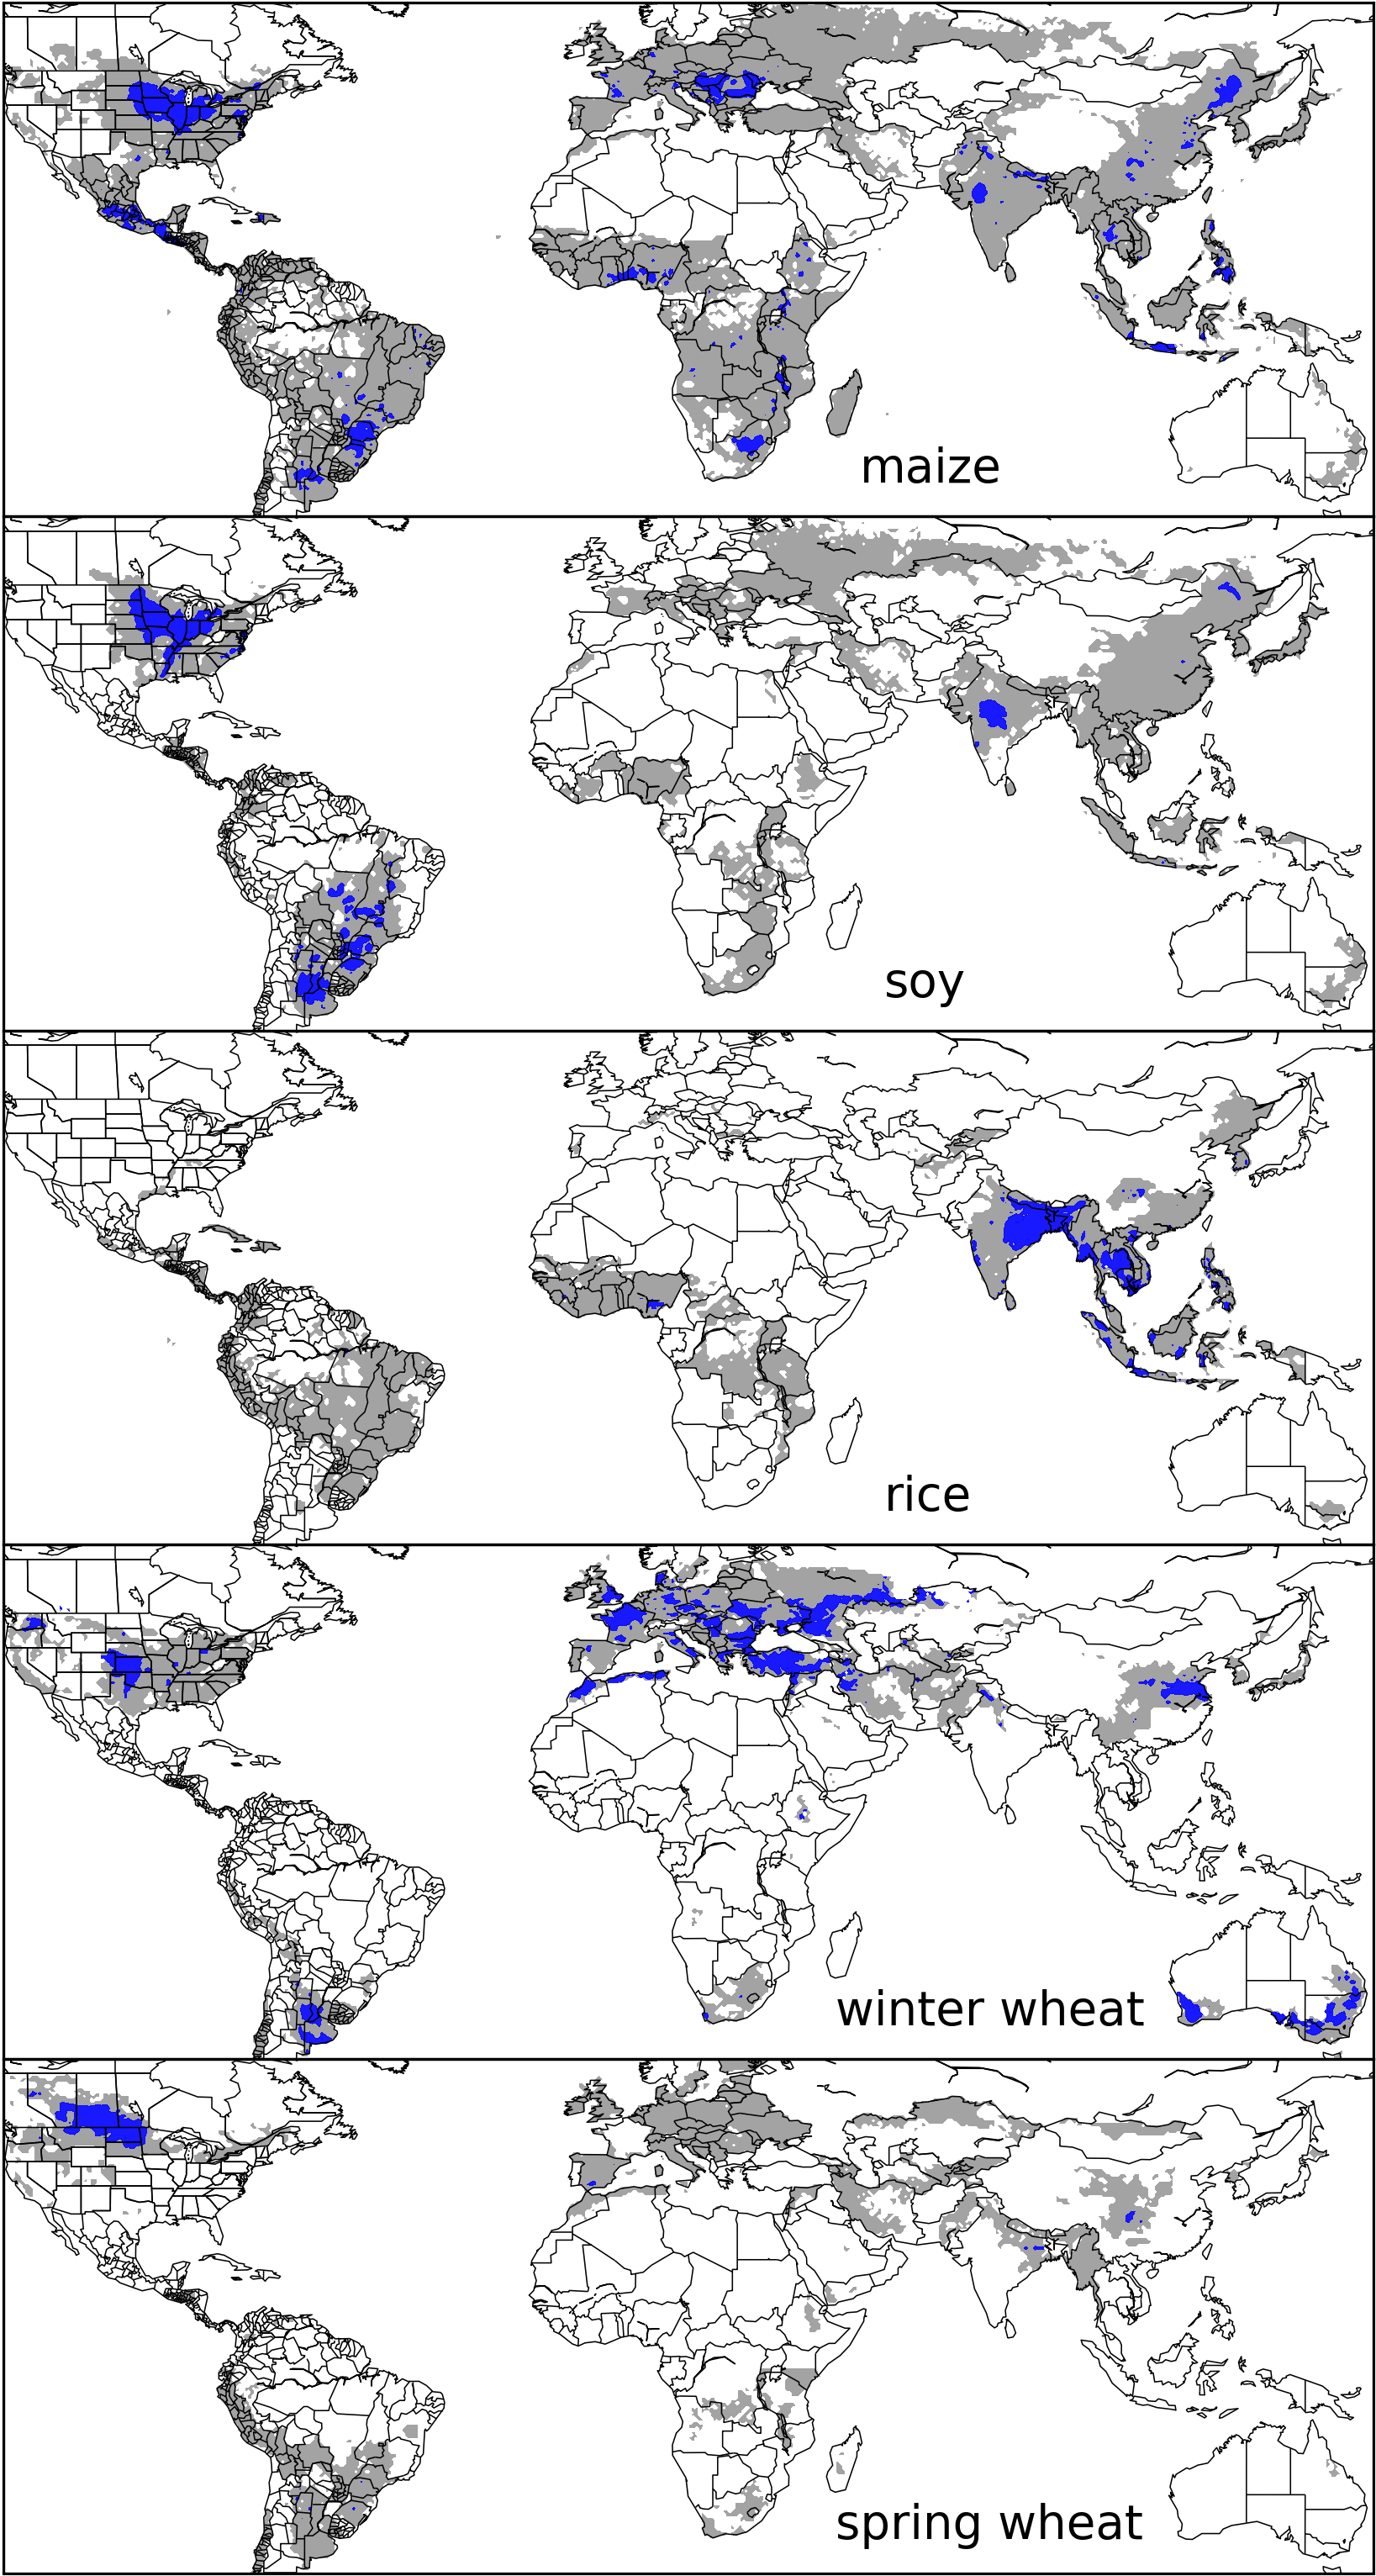
\includegraphics[width=8.3cm]{figures/croparea.png}
   \caption{Presently cultivated area for rainfed crops. Blue indicates grid cells with more that 20,000 hectares ($\sim$10\% of an equatorial grid cell). 
   Gray contour shows area with more that 10 hectares cultivated. Cultivated areas for maize, rice, and soy are taken from the MIRCA2000 (``monthly irrigated and rainfed crop areas around the year 2000'') dataset \citep{Portmann2010}. 
   Areas for winter and spring wheat areas are adapted from MIRCA2000 data and sorted by growing period. 
   For analogous figure of irrigated crops, see Figure S1.}
   \label{fig:crop_area}
\end{figure}

Coverage extends considerably outside currently cultivated areas because cultivation will likely shift under climate change.  
However, areas are not simulated in some cases if they are assumed to remain non-arable even under an extreme climate change; these regions include Greenland, far-northern Canada, Siberia, Antarctica, the Gobi and Sahara Deserts, and central Australia. 
All models produce as output crop yields (tons ha$^{-1}$ year$^{-1}$) for each 0.5 degree grid cell. Because both yields and yield changes vary substantially across models and across grid cells, we primarily analyze relative change from a baseline. 
We take as the baseline the scenario with historical climatology (i.e.\ T and P changes of 0), C of 360 ppm, and applied N at 200 kg ha$^-1$. 
The GGCMI Phase II simulations are designed for evaluating changes in yield but not absolute yields, since they omit detailed calibrations. 
To provide some evaluation of the skill of the process-based models used, we repeat the evaluation exercises of \citet{muller_global_2017} for GGCMI Phase I.

\subsubsection{Input data and harmonization}

In most cases, historical daily climate inputs are taken from the 0.5 degree NASA AgMERRA daily gridded re-analysis product specifically designed for agricultural modeling, with satellite-corrected precipitation \citep{Ruane2015}, but two models (JULES and PROMET) require sub-daily input data and use alternative baseline climate inputs (WFDEI \citep{weedon2014wfdei} and ERA-Interim \citep{dee2011era}, respectively). 

Temperature perturbations are applied as absolute offsets from the daily mean, minimum, and maximum temperature time series for each grid cell.
Precipitation perturbations are applied as fractional changes at the grid cell level, and [CO$_2$] and nitrogen levels are specified as discrete values applied uniformly over all grid cells. 
No other N inputs are assumed (i.e. no atmospheric deposition), but soil mineralization can supply additional plant-available N, which can vary by model. 

\begin{table}[t]
\caption{GGCMI Phase II input levels. Temperature and precipitation values indicate the perturbations from the historical climatology. W-percentage does not apply to the irrigated (W$_{inf}$) simulations, which are all simulated at the maximum beneficial levels of water. Bold font indicates the `baseline' historical level. One model provided simulations at the T + 5 level. See Figure S3 in the supplement for number of simulations associated with each combination of input levels.}
\label{table:inputs} 
    \begin{tabular}{lcc} 
        \tophline \vspace{1mm}
        \textbf{Input variable} & \textbf{Tested range} & \textbf{Unit} \\ \middlehline \vspace{1mm}
        [CO$_2$] (C) & \textbf{360}, 510, 660, 810 & ppm\\ \middlehline \vspace{1mm}
        Temperature (T) & -1, \textbf{0}, 1, 2, 3, 4, 6 & $^{\circ}$C\\ \middlehline \vspace{1mm}
        Precipitation (W) & -50, -30, -20, -10, \textbf{0}, & \% \\
        {} & 10, 20, 30, (and W$_{inf}$) & {} \\ \middlehline \vspace{1mm}
        Applied nitrogen (N) & 10, 60, \textbf{200} & kg ha$^{-1}$ \\ \middlehline \vspace{1mm}
        Adaptation (A) & \textbf{A0: none}, A1: new cultivar to maintain original growing season length & -\\ \bottomhline
    \end{tabular}\\
\end{table}

Growing seasons are standardized across models (with assumptions based on \citet{Sacks2010} and \citet{Portmann2008, Portmann2010}), but vary by crop and by location on the globe. 
For example, maize is sown in March in Spain, in July in Indonesia, and in December in Namibia. 
Only growing seasons for rainfed systems are used in GGCMI phase II, as full irrigation is treated as one perturbation level in the W dimension (``Winf'').
Growing seasons for maize, rice, and soybean have been used from phase 1 \citep{Elliott2015}, but wheat was separated into spring wheat (swh) and winter wheat (wwh) so that new growing season data had to be provided. 
For this, wheat crop calendars were separated following simple rules. 
The SAGE crop calendar \citep{Sacks2010} provides separate spring and winter cropping seasons. 
This was used as primary source of information, as for the other crops \citep{Elliott2015}. 
In areas, where no SAGE crop calendar information is available, the MIRCA2000 crop calendar \citep{Portmann2010} was used. Wheat growing seasons were assigned to winter wheat if 
\begin{itemize}
\item the mean monthly temperature is below freezing point (<0$^\circ$C) at most for 5 months per year,
\item the coldest 3 months of a year are below 10$^\circ$C
\item the season starts after the warmest or before the coldest month of the year on the northern hemisphere, or
\item the season starts after the warmest and before the coldest month of the year on the southern hemisphere
\end{itemize}
and were assigned to spring wheat otherwise. 
For areas where also not MIRCA2000 crop calendar was available, simulated LPJmL growing seasons \citep{waha2012climate} were used as in phase 1 \citep{Elliott2015}, applying the same rules as for MIRCA2000 to distinguish spring wheat from winter wheat seasons.

As per convention, N fertilizer is to be applied in two doses to reduce losses to the environment. For simplicity, the first half of the total fertilizer input is to be applied at sowing and the other half is to be applied on day 40 after sowing for all crops except for winter wheat. For winter wheat, the application date for the second N fertilizer application was provided, because the length of dormancy during winter can be quite variable across regions. The second fertilization date for winter wheat was set to the middle day of the first month with average temperatures above 5$^\circ$C after sowing with a minimum distance to the maturity date of 50 days and to planting of 40 days.

All stresses are disabled other than factors related to nitrogen, temperature, and water (e.g.\ alkalinity, salinity, non-nitrogen nutrients). 
No additional nitrogen inputs, such as atmospheric deposition, are considered, but some model treatments of soil organic matter allows additional nitrogen release through mineralization. 
%See \citet{Elliott2015} for further details on model setup for intercomparison in the GGCMI protocol. 


\subsubsection{Output data conventions and file names}

All output data is supplied as netCDF version 4 files as in GGCMI phase 1 \citep{Elliott2015} following a similar naming convention. As the ISIMIP file naming convention now includes the identifier $global$ to distinguish regional from global model output \citep{frieler2017assessing}, we follow that convention here as well:

$[model]\_[climate]\_hist\_fullharm\_[irrig.scenario]\_[variable]\_[crop]\_global\_annual\_[start-year]\_[end-year].nc4$

\noindent where $[model]$ is the GGCM name, $[climate]$ is the original climate input data set (typically AgMERRA), $[irrig.scenario]$ is the irrigation setting ("firr" for fully irrigated and "noirr" for fully rainfed), $[variable]$ is the output variable (see Table \ref{table:outputs}), $[crop]$ is the crop abbreviation ("mai" for maize, "ric" for rice, "soy" for soybean, "swh" for spring wheat, "wwh" for winter wheat), $[start-year]\_[end-year]$ specify the first and last year recorded on file. 
The entire file name needs to be in small caps. 
The first entry in the file is the result of the first simulated cropping cycle that is entirely within the given climate input. 
For AgMERRA, where the first year provided is 1980, the first harvest record is thus of 1980, when the prescribed sowing and harvest dates are in 1980 (e.g. sowing in March and harvest in September 1980) but is of 1981 if sowing is later in a calendar year than harvest (e.g. sowing in September 1980 and harvest in March 1981). 
To avoid distortions in harvest events, output files report the sequence of growing periods rather than calendar years. 
In most cases, this is equivalent, as there is always only one sowing event per calendar year.
As harvest events are internally determined as a function of mostly temperature, these can vary between individual years. 
If harvest events are around the end of the calendar year (Dec. 31), reported values could contain 2 (one in early January and one in late December), 1 (normal) or none (last was in December of previous year and next is in January of the following year) harvest event if reported per calendar year.
As in phase 1, all output data need to be provided on a regular geographic grid, spanning latitudes from -89.75 to 89.75$^{\circ}$ and longitudes from -179.75 to 179.75$^{\circ}$ (referring to the center of each grid cell). 
Missing values, i.e. where no crop growth has been simulated, such as ocean grid cells, need to be reported as 1.e+20f whereas crop failure should be reported as zero yield. 
Following NetCDF standards, latitude, longitude and time must be included as separate variables in ascending order.
Units of these axes are "degrees north", "degrees east", and "growing seasons since YYYY-01-01 00:00:00", where YYYY indicates the first year (1980 for AgMERRA).

Next to simulated yield data, crop modelers are requested to provide additional output variables (Table \ref{table:outputs}). 

\begin{table}[]
\caption{Main output variables requested per crop. Mandatory outputs (if available in that GGCM) in \textbf{bold}. Some models provide additional variables, such as more detailed separation of total nitrogen losses. }
\label{table:outputs}
\begin{tabular}{lll}
        \tophline \vspace{1mm}
Variable                                & variable name             & units \\
\middlehline \vspace{1mm}
\textbf{Yield}                                   & \textbf{yield\_<crop>}     & \textbf{t ha$^{-1}$ yr$^{-1}$ (dry matter)}\\
\textbf{Total above ground biomass yield}        & \textbf{biom\_<crop>}      & \textbf{t ha$^{-1}$ yr$^{-1}$ (dry matter)}\\
\textbf{Actual planting date}                    & \textbf{plant-day\_<crop>} & \textbf{day of year}\\
\textbf{Anthesis date}                           & \textbf{anth-day\_<crop>}  & \textbf{days from planting} \\
\textbf{Maturity date}                           & \textbf{maty-day\_<crop>}  & \textbf{days from planting}\\
\textbf{Applied irrigation water}                & \textbf{pirrww\_<crop>}    & \textbf{mm yr$^{-1}$} \\
\textbf{Evapotranspiration (growing season sum)} & \textbf{etransp\_<crop>}   & \textbf{mm yr$^{-1}$ (firr scenarios only)}\\ \middlehline
Transpiration (growing season sum)                       & transp\_<crop>    & mm yr$^{-1}$ \\
Evaporation (growing season sum)                         & evap\_<crop>      & mm yr$^{-1}$ \\
Runoff (total growing season sum, subsurface + surface)  & runoff\_<crop>    & mm yr$^{-1}$                    \\
Total available soil moisture in root zone *             & trzpah2o\_<crop>  & mm yr$^{-1}$                    \\
Total root biomass                                       & rootm\_<crop>     & t ha$^{-1}$ yr$^{-1}$ (dry matter)  \\
Total Nr uptake (total growing season sum)               & tnrup\_<crop>     & kg ha$^{-1}$ yr$^{-1}$              \\
Total Nr inputs (total growing season sum)               & tnrin\_<crop>     & kg ha$^{-1}$ yr$^{-1}$              \\
Total Nr losses (total growing season sum)               & tnrloss\_<crop>   & kg ha$^{-1}$ yr$^{-1}$              \\
Gross primary production (GPP)                           & gpp\_<crop>       & gC m$^{-2}$ yr$^{-1}$               \\
Net primary production (NPP)                             & npp\_<crop>       & gC m$^{-2}$ yr$^{-1}$               \\
CO$_2$ response scaler on NPP                            & co2npp\_<crop>    & - \{0..inf\}                \\
water response scaler on NPP                             & h2onpp\_<crop>    & - \{0..1\}                  \\
temperature response scaler on NPP                       & tnpp\_<crop>      & - \{0..1\}                  \\
Nr response scaler on NPP                                & nrnpp\_<crop>     & - \{0..1\}                  \\
Other nutrient response scaler on NPP                    & ornpp\_<crop>     & - \{0..1\}                  \\
CO$_2$ response scaler on transpiration                  & co2trans\_<crop>  & - \{0..1\}                  \\
maximum stress response scaler                           & maxstress\_<crop> & - \{0..1\}                  \\
Maximum LAI                                              & laimax\_<crop>    & m$^{2}$ m$^{-2}$           \\        
\bottomhline
* growing season sum, basis for computing average soil moisture & {} & {} \\
\end{tabular}
\end{table}

A script for initial data quality screening has been provided to the modeling groups so that these could test plausible data range and spatial coverage prior to data submission.


\subsection{Models contributing}

Given the substantial computational requirements for participation in GGCMI Phase II with 756 (A0) + 648 (A1) global 31-year simulations for 5 different crops, we specified different participation tiers to allow submission of smaller sub-sets. 
These subsets were designed as orthogonal samples across the 4 dimensions of the CTWN space. 
These are designed by combinations of selected pairs in the CxN space (all 12 vs. 4 pairs: C360\_N10, C360\_N200, C660\_N60, C810\_N200) and the TxW space:
\begin{itemize}
\item a \textit{minimum set} with an orthogonal, stratified 9-step sampling (T-1W-10, T0W10, T1W-30, T2W-50, T2W20, T3W30, T4W0, T4Winf, T6W-20)
\item a \textit{reduced set} of alternating combinations, which uses different W for even Ts than for odd Ts. For even Ts (i.e. T0,T2,T4,T6), we use W = -50,-20,0,+30 = 4*4, for odd Ts (i.e. T-1,T1,T3) , we use W = -30, -10, +10, +30, inf = 3*5,
\item and the \textit{full set} (all 7Tx9W)
\end{itemize}

The different participation levels are thus defined by combining the CxN sets with the TxW sets:

\begin{itemize}
\item \textbf{full}: all 756 (648) A0 (A1) simulations (all 12 CxN * all 63 TxW)
\item \textbf{high tier}: 362 simulations (all 12 CxN combinations * \textit{reduced} TxW set of 31 combinations)
\item \textbf{mid tier}: 124 simulations (low 4 CxN combinations * \textit{reduced} TxW set of 31 combinations)
\item \textbf{low tier}: 36 simulations (low 4 CxN combinations * \textit{minimum} TxW set of 9 combinations)
\end{itemize}

\begin{table*}[t]
\caption{Models included in GGCMI Phase II and the number of C, T, W, and N simulations that each performs, with 756 as the maximum for A0 (no adaptation) and 648 as the maximum for A1 (maintaining growing season adaptation). 
``N-Dim.'' indicates whether the simulations include varying nitrogen levels. Two models provide only one nitrogen level. 
All models provide the same set of simulations across all modeled crops, but some omit individual crops. (For example, APSIM does not simulate winter wheat.)}
\label{table:models}
	\begin{tabular}{p{6cm} p{1cm} p{1cm} p{1cm} p{1cm} p{1cm} p{1cm} p{1.9cm}}
        \tophline
        {\textbf{Model (Key Citations)}}&{\textbf{Maize}}&{\textbf{Soy}}&{\textbf{Rice}}&{\textbf{Winter wheat}}&{\textbf{Spring wheat}}&{\textbf{N dim.}}&{\textbf{Sims per crop (A0 / A1}}\\ \middlehline
        {\textbf{APSIM-UGOE},   \citet{KEATING2003267, HOLZWORTH2014327}} & {X} & {X} & {X} & {--} & {X} & {X} & {44 / 36}\\ \middlehline
        {\textbf{CARAIB},       \citet{Dury2011, Pirttioja2015}} & {X} & {X} & {X} & {X} & {X} & {--} & {252 / 216}\\ \middlehline
        {\textbf{EPIC-IIASA},   \citet{BALKOVIC2014}} & {X} & {X} & {X} & {X} & {X} & {X} & {39 / 0}\\  \middlehline
        {\textbf{EPIC-TAMU},    \citet{Izaurralde06}} & {X} & {X} & {X} & {X} & {X} & {X} & {765 / 648}\\ \middlehline
        {\textbf{JULES},        \citet{Osborne2015, Williams2015, Williams2017}} & {X} & {X} & {X} & {--} & {X} & {--} & {252 / 0}\\ \middlehline
        {\textbf{GEPIC},        \citet{LIU2007478, FOLBERTH201221}} & {X} & {X} & {X} & {X} & {X} & {X} & {430 / 181}\\ \middlehline
        {\textbf{LPJ-GUESS},    \citet{Lindeskog2013, Olin2015}} & {X} & {--} & {--} & {X} & {X} & {X} & {756 / 648}\\  \middlehline
        {\textbf{LPJmL},        \citet{von_Bloh_implementing_2018}} & {X} & {X} & {X} & {X} & {X} & {X} & {756 / 648}\\ \middlehline
        {\textbf{ORCHIDEE-crop},\citet{Wu2016}} & {X} & {--} & {X} & {X} & {--} & {X} & {33 / 0}\\ \middlehline
        {\textbf{pDSSAT},       \citet{Elliott2014b, JONES2003235}} & {X} & {X} & {X} & {X} & {X} & {X} & {756 / 648}\\ \middlehline
        {\textbf{PEPIC},        \citet{LIU2016164, LIU2016}} & {X} & {X} & {X} & {X} & {X} & {X} & {149 / 121}\\ \middlehline
        {\textbf{PROMET},       \citet{Hank2015, MAUSER2015}} & {X} & {X} & {X} & {X} & {X} & {X} & {261 / 232}\\ \middlehline
        {Totals} & {12} & {10} & {11} & {11} & {11} & {10} & {5240 | 3378}\\
        \bottomhline
    \end{tabular}
\end{table*}


The 12 models included in GGCMI Phase II are all process-based crop models that are widely used in impacts assessments (Table \ref{table:models}). 
Although some models share a common base (e.g.\ the LPJ family or the EPIC family of models), they have subsequently developed independently. 
Differences in model structure mean that several key factors are not standardized across the experiment, such as carry-over effects across growing years including residue management and soil moisture, and the extent of simulated area for different crops. 
Not all modeling teams provide the full simulation protocol, for instance, CARIAB and JULES do not simulate the nitrogen dimension and some crops are not parameterized in each model (see Table \ref{table:models} for details). 
%Note that the three models that provide less than 50 simulations are excluded from the emulator analysis (APSIM-UGOE, EPIC-IIASA, and ORCHIDEE-crop).

%%%%%%%%%%%%%%%%%%%%%%%%%%%%%%%%%%%%%%%%%%%%%%%%%%%%%%%%%%%%%%%
%%%%%%%%%%%%%%%%%%%%%%%%%%%%%%%%%%%%%%%%%%%%%%%%%%%%%%%%%%%%%%%
%%%%%%%%%%%%%%%%%%%%%%%%%%%%%%%%%%%%%%%%%%%%%%%%%%%%%%%%%%%%%%%
\section{Simulation Assessment}
\label{S:3}

\begin{figure*}[ht]
    \centering
    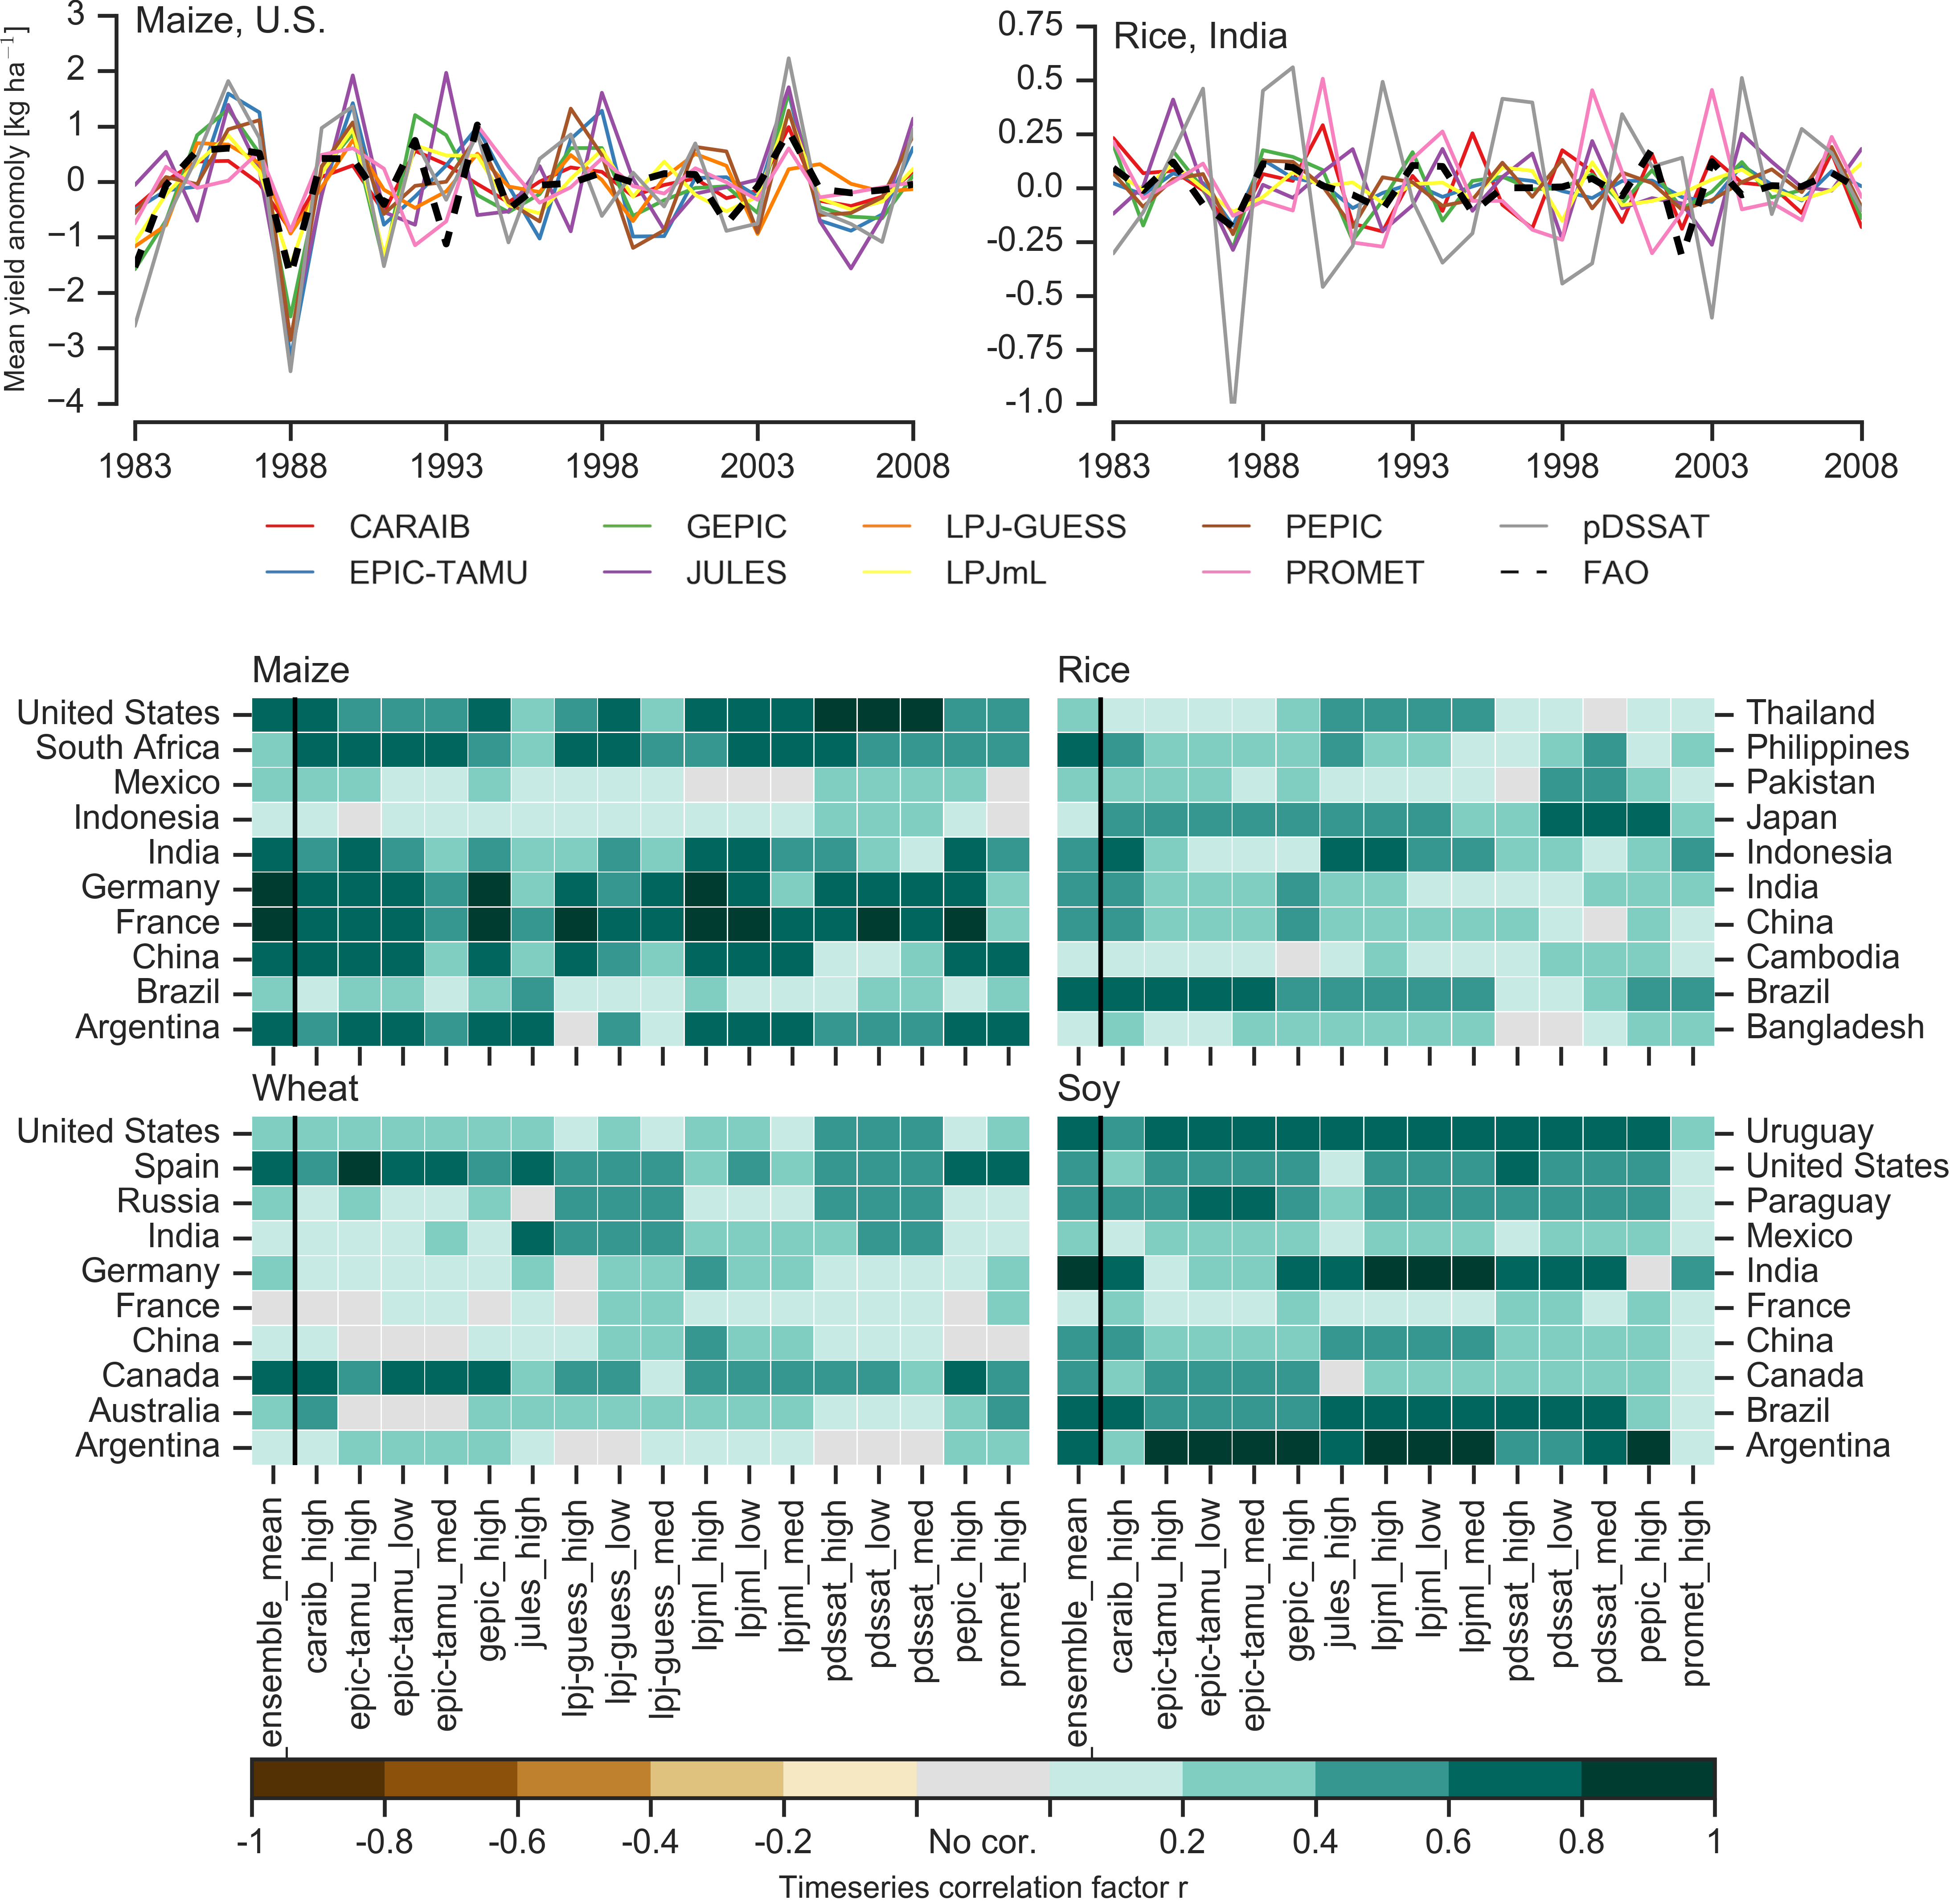
\includegraphics[width=14cm]{figures/Agformet_validation.png}
    \caption{Time series of correlation coefficients between simulated crop yield and FAO data \citep{FAOSTAT} at the country level. 
    The top panels indicate two example cases: US maize (a good case), and rice in India (mixed case), both for the high nitrogen application case. 
    The heatmaps illustrate the Pearson $r$ correlation coefficient between the detrended simulation mean yield at the country level compared to the detrended FAO yield data for the top producing countries for each crop with continuous FAO data over the 1981-2010 period. 
    Models that provided different nitrogen application levels are shown with low, med, and high label (models that did not simulate different nitrogen levels are analogous to a high nitrogen application level). 
    The ensemble mean yield is also correlated with the FAO data (not the mean of the correlations). 
    Wheat contains both spring wheat and winter wheat simulations where supplied, else one or the other (see Table 2). 
    The Pearson r correlation coefficients are similar to those of GGCMI Phase I, with reasonable fidelity at capturing year-over-year variation, with differences by region and crop stronger than difference between models as indicated by more horizontal bars than vertical bars of the same color.}
    \label{fig:simulation_val}
\end{figure*}

The \citet{muller_global_2017} procedure evaluates response to year-to-year temperature and precipitation variations in a control run driven by historical climate and compares it to detrended historical yields from the FAO \citep{FAOSTAT} by calculating the Pearson product moment correlation coefficient. 
The procedure is sensitive to the detrending method and the area mask used to aggregate yields. Here we use a 5-year running mean removal and the MICRA area mask for aggregation. 
In some cases the time series are shifted by one year to account for errors in FAO or model year reporting. The procedure offers no means of assessing CO$_2$ fertilization, since [CO$_2$] has been relatively constant over the historical data collection period. 
Nitrogen introduces another source of uncertainty into the analysis, since the GGCMI Phase II runs impose fixed, uniform nitrogen application levels that are not realistic for individual countries. 
We evaluate up to three control runs for each model, since some modeling groups provide historical runs for three different nitrogen levels. 

Results are similar to those of GGCMI Phase I, with reasonable fidelity at capturing year-over-year variation, with differences by region and crop stronger than difference between models. 
(That is, Figure \ref{fig:simulation_val} shows more similarity in horizontal than vertical bars.) 
No single model is dominant, with each model providing near best-in-class performance in at least one location-crop combination. 
For example, maize in the United States is consistently well-simulated while maize in Indonesia is problematic (mean Pearson correlation coefficients of 0.68 and 0.18, respectively). 
In some cases, especially in the developing world, low correlation coefficients may indicate not only model failure but also problems in FAO yield data. 

In general, correlation coefficients in GGCMI Phase II are slightly below those of Phase I, likely because of unrealistic nitrogen levels, lack of country level calibration in some models, and restriction to only the MICRA aggregation mask in this study. 
(Compare Figure \ref{fig:simulation_val} to \citet{muller_global_2017} Figures 1--4 and 6.)  
Additionally, the time period used in this case is slightly different from the time period used in \citet{muller_global_2017}. 
Note that in this methodology, simulations of crops with low year-to-year variability such as irrigated rice and wheat will tend to score more poorly than those with higher variability.

Some models do show particular strength for particular crops. 
For example, the EPIC family of models, and especially the EPIC-TAMU model, perform particularly well for soy across all regions. 
In other cases a model has particular strength in only certain crop and region combinations. 
For example, the strongest correlation coefficient in Figure \ref{fig:simulation_val} is that for the pDSSAT model for maize in the U.S. (the example crop-model-location used in many example figures in this paper), but pDSSAT slightly under performs for maize in other regions. 
These model assessment results are similar to those for GGCMI Phase I in \citet{muller_global_2017}.


%%%%%%%%%%%%%%%%%%%%%%%%%%%%%%%%%%%%%%%%%%%%%%%%%%%%%%%%%%%%%%%
%%%%%%%%%%%%%%%%%%%%%%%%%%%%%%%%%%%%%%%%%%%%%%%%%%%%%%%%%%%%%%%
%%%%%%%%%%%%%%%%%%%%%%%%%%%%%%%%%%%%%%%%%%%%%%%%%%%%%%%%%%%%%%%
\section{Results}

\label{S:4}
\begin{figure*}[ht]
\centering
   \includegraphics[width=14cm]{figures/baselinecomp_yield_3.png} 
   \caption{Illustration of the spatial pattern of potential yields and potential yield changes in the GGCMI Phase II ensemble, for three major crops. 
   Left column (a) shows multi-model mean climatological yields for the baseline scenario for (top--bottom) rainfed maize, soy, and rice. Wheat shows a qualitatively similar response, see Figure S16 in the supplemental material. 
   White stippling indicates areas where these crops are not currently cultivated. 
   Absence of cultivation aligns well with the lowest yield contour (0-2 ton ha$^{-1}$). 
   Right column (b) shows the multi-model mean fractional yield change in the extreme T + 4 $^{\circ}$C scenario (with other inputs at baseline values). 
   Areas without hatching or stippling are those where confidence in projections is high: the multi-model mean fractional change exceeds two standard deviations of the ensemble. ($\Delta > 2\sigma$). 
   Hatching indicates areas of low confidence ($\Delta < 1 \sigma$), and stippling areas of medium confidence ($1 \sigma < \Delta < 2 \sigma$). 
   Crop model results in cold areas, where yield impacts are on average positive, also have the highest uncertainty.}
   \label{fig:maizesoybaseline}
\end{figure*}

\begin{figure*}[ht]
\centering
   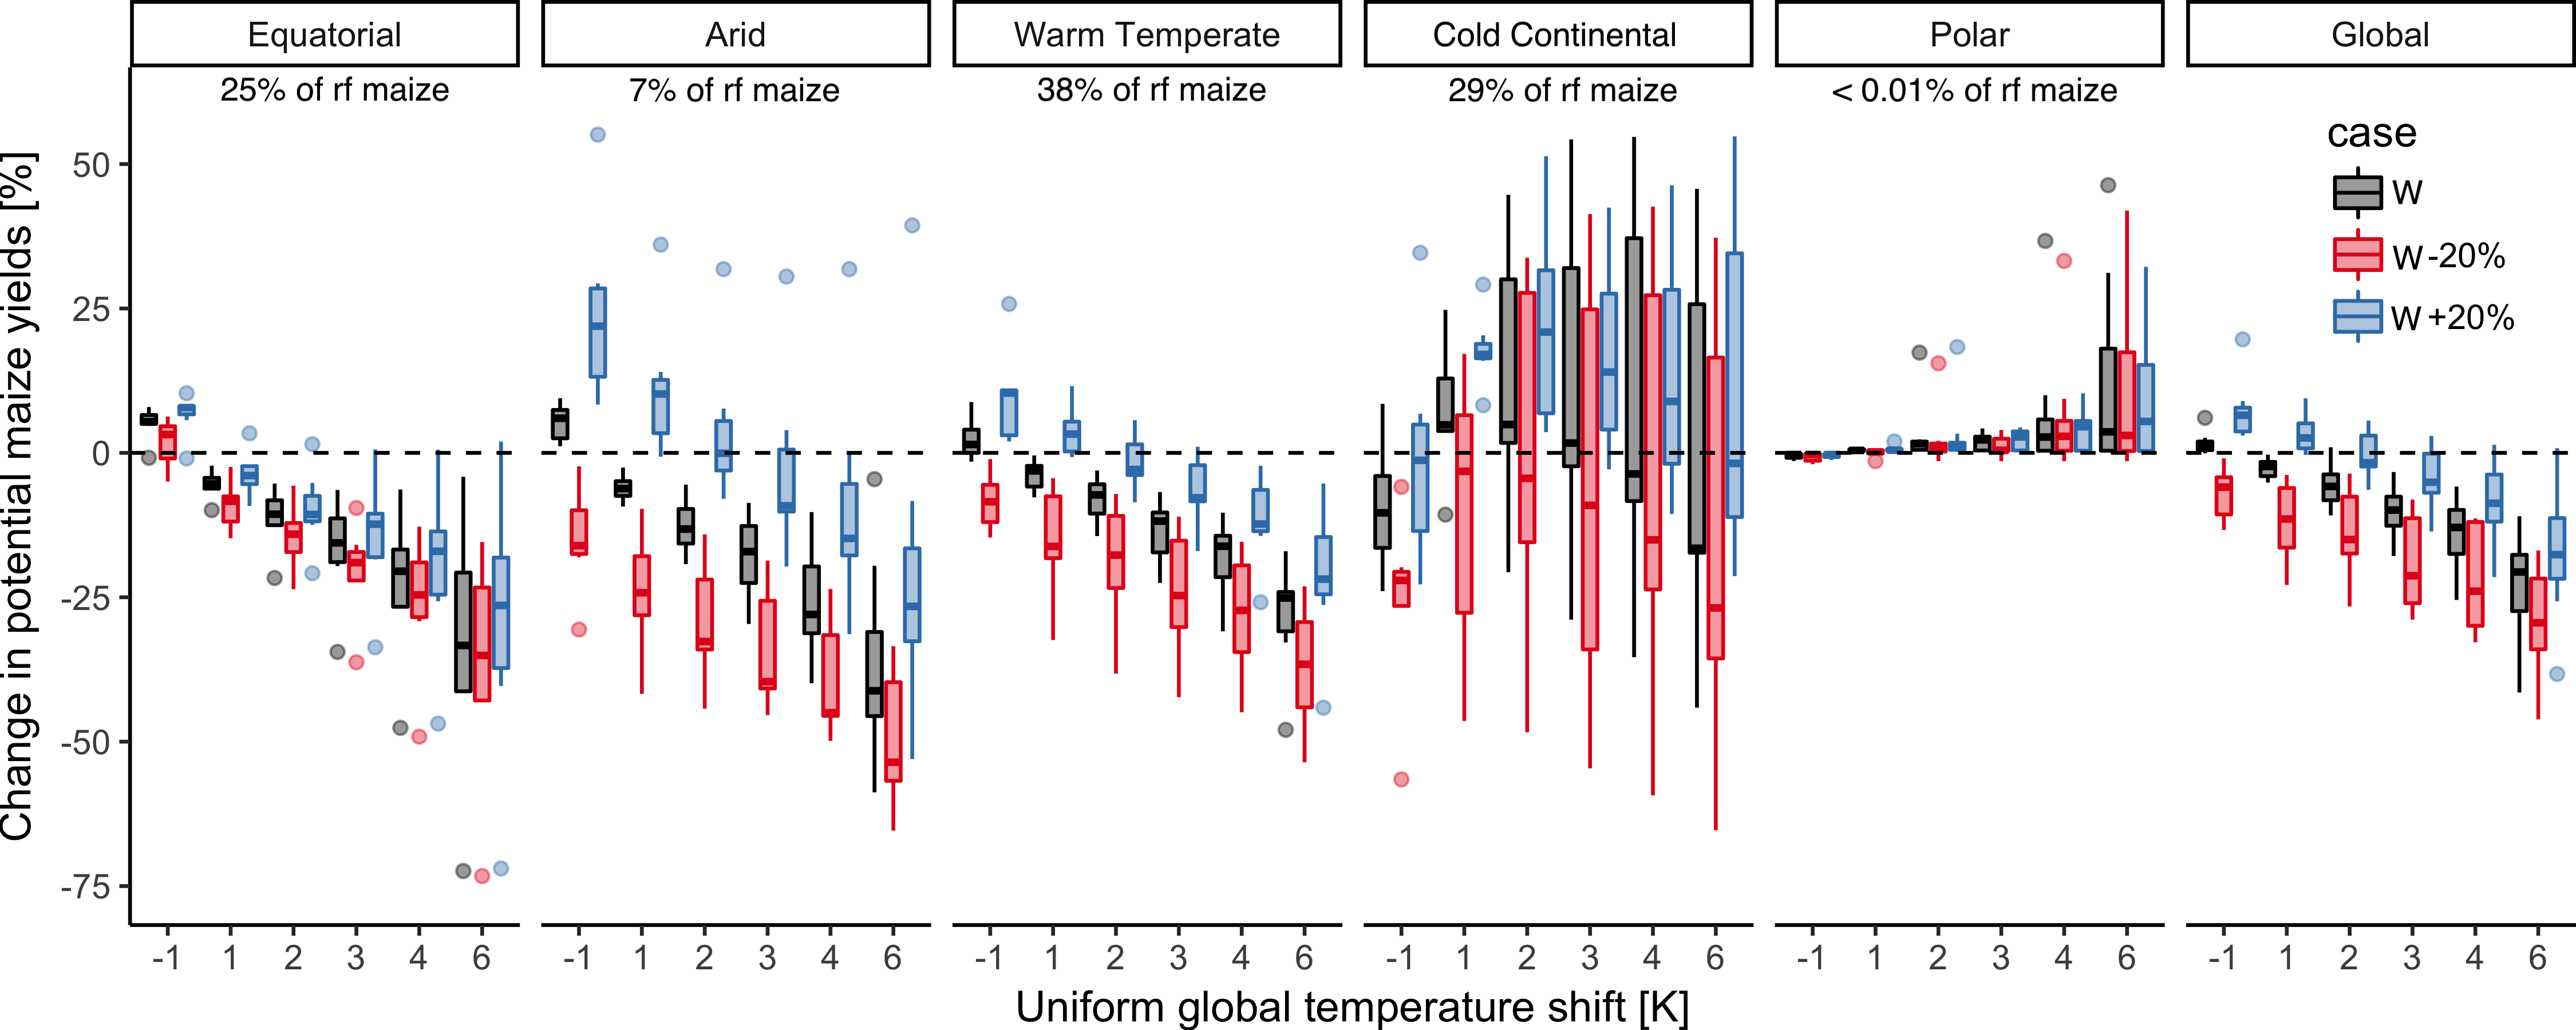
\includegraphics[width=15cm]{figures/global_sim_CG.png}
   \caption{Illustration of the distribution of regional yield changes across the multi-model ensemble, split by K\"{o}ppen-Geiger climate regions \citep{rubel2010}. 
   We show responses of a single crop (rainfed maize) to applied uniform temperature perturbations, for three discrete precipitation perturbation levels ( -20\%, 0\%, and +20\%), with [CO$_2$] and nitrogen held constant at baseline values (360 pmm and 200 kg ha$^{-1}$ yr$^{-1}$). 
	Y-axis is fractional change in the regional average climatological potential yield relative to the baseline. Box-and-whiskers plots show distribution across models, with median marked; edges are first and third quartiles, i.e.\ box height is the interquartile range (IQR). 
	If all models like within 1.5$\cdot$IQR then whiskers extend to maximum and minimum of simulations, else the outlier is shown separately. Outliers in the tropics (strong negative impact of temperature increases) are the pDSSAT model; outliers in the high-rainfall case (strong positive impact of precipitation increases) are the JULES model. 
	Figure shows all modeled land area; see Figure S4 in the supplemental material for currently-cultivated land and Figure S5 for other crops. Panel text gives the percentage of rainfed maize presently cultivated in each climate zone \citep[data from][]{Portmann2010}. 
	Note that \citet{rubel2010} use the name `Snow' rather than `Cold continental'. 
	Outside high-latitude regions ('Cold continental' and `Polar'), models generally agree, with projected declines under increasing temperatures larger than inter-model variance. 
	The right panel (Global) shows yield responses to a globally uniform temperature shift; note that these results are not directly comparable to simulations of more realistic climate scenarios.}
   \label{fig:globesim}
\end{figure*}

\begin{figure*}[ht]
\centering
   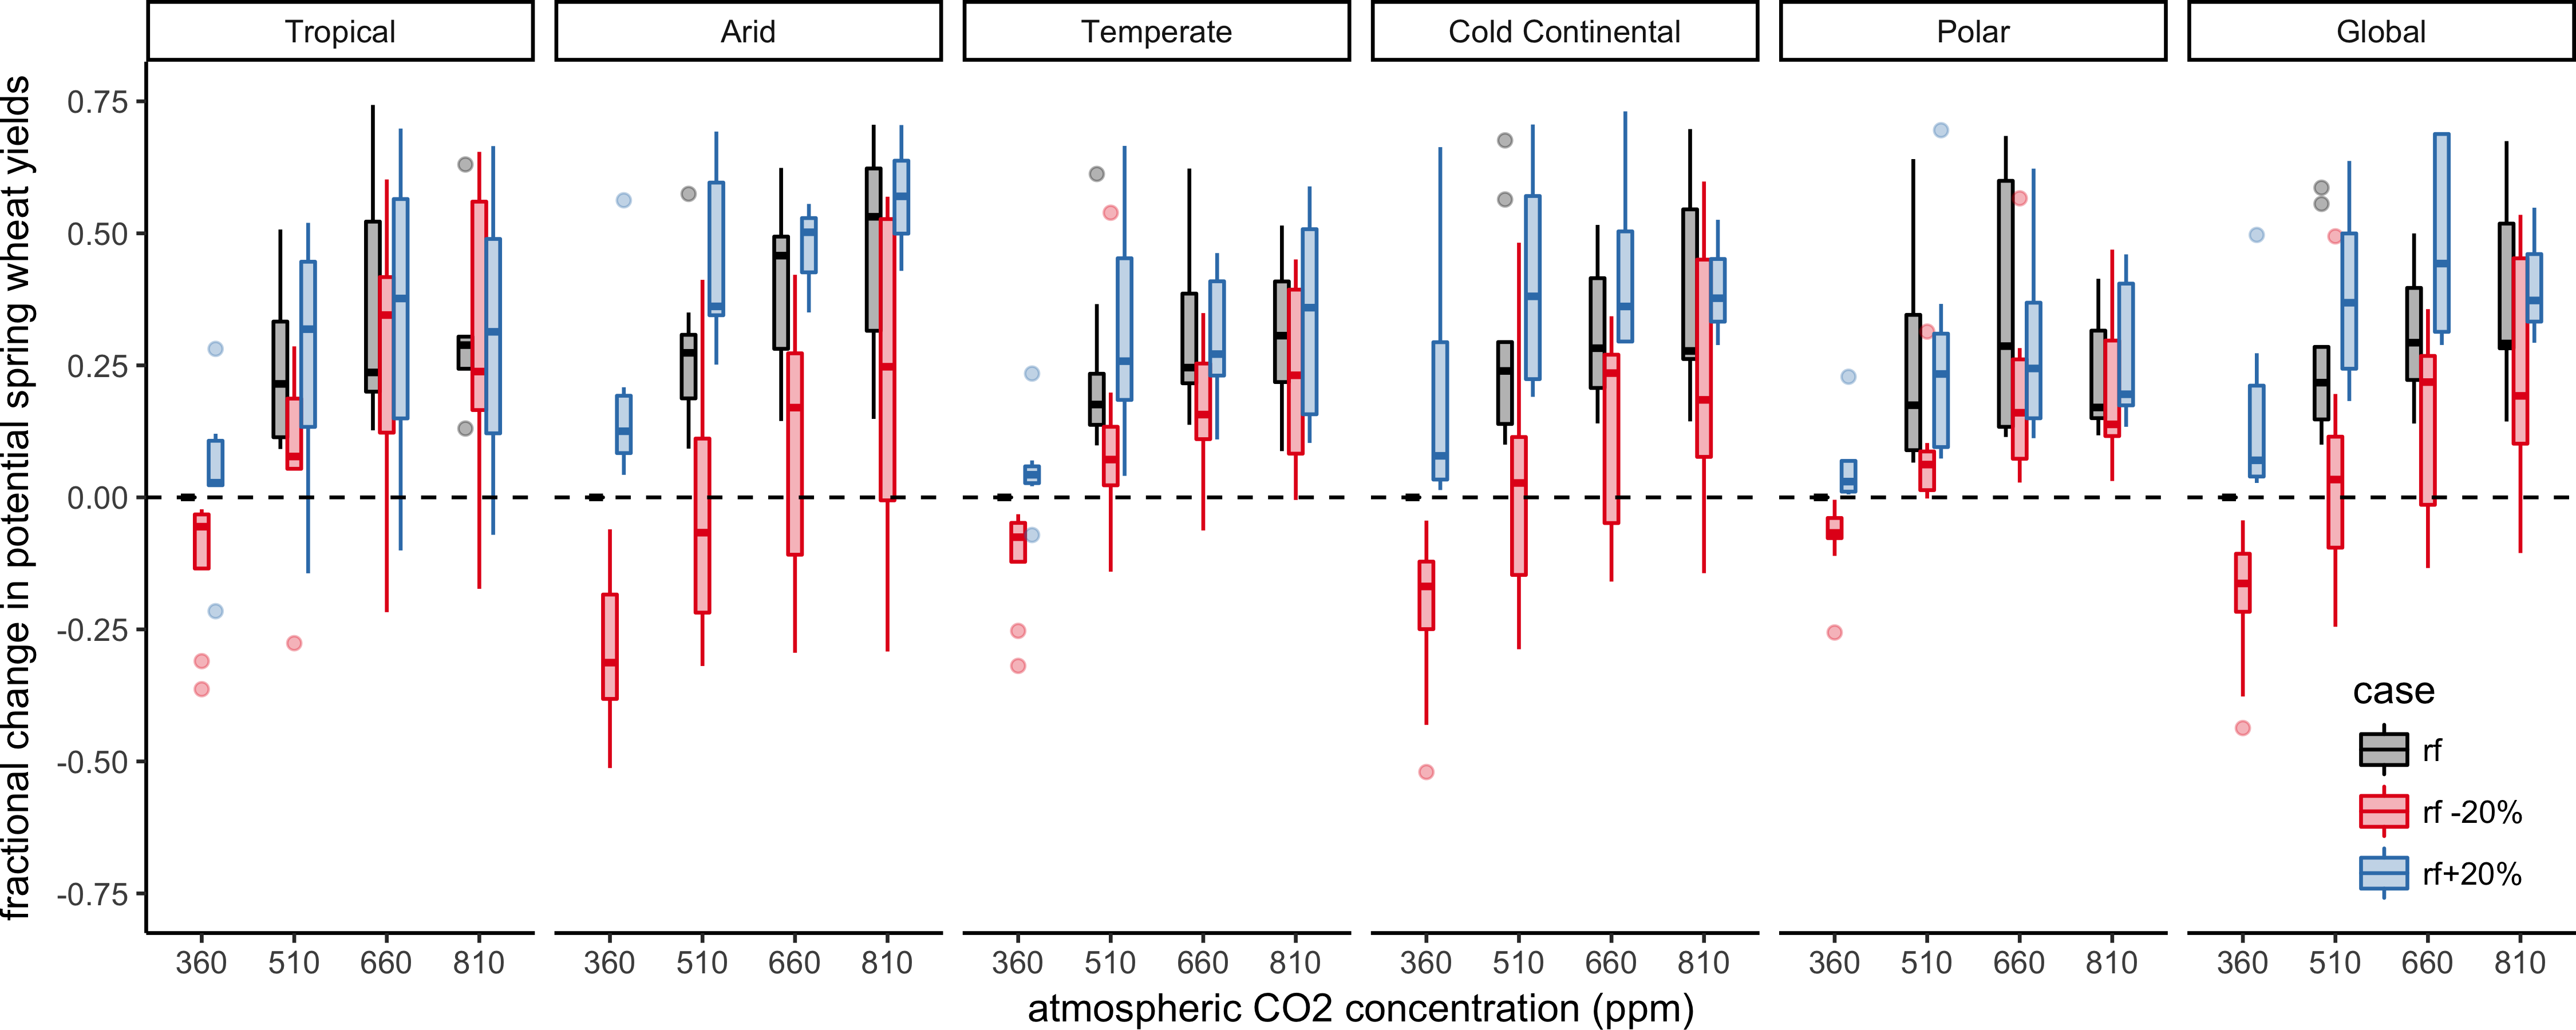
\includegraphics[width=15cm]{figures/swh_sim_CG_C.png}
   \caption{Illustration of the distribution of regional yield changes across the multi-model ensemble, split by K\"{o}ppen-Geiger climate regions for spring wheat. Same as Figure \ref{fig:globesim} except atmospheric carbon dioxide is varied. Two different water specifications (precipitation -20\% and precipitation +20\%) are shown in colors.}
   \label{fig:globesim_C}
\end{figure*}

\begin{figure*}[ht]
\centering
   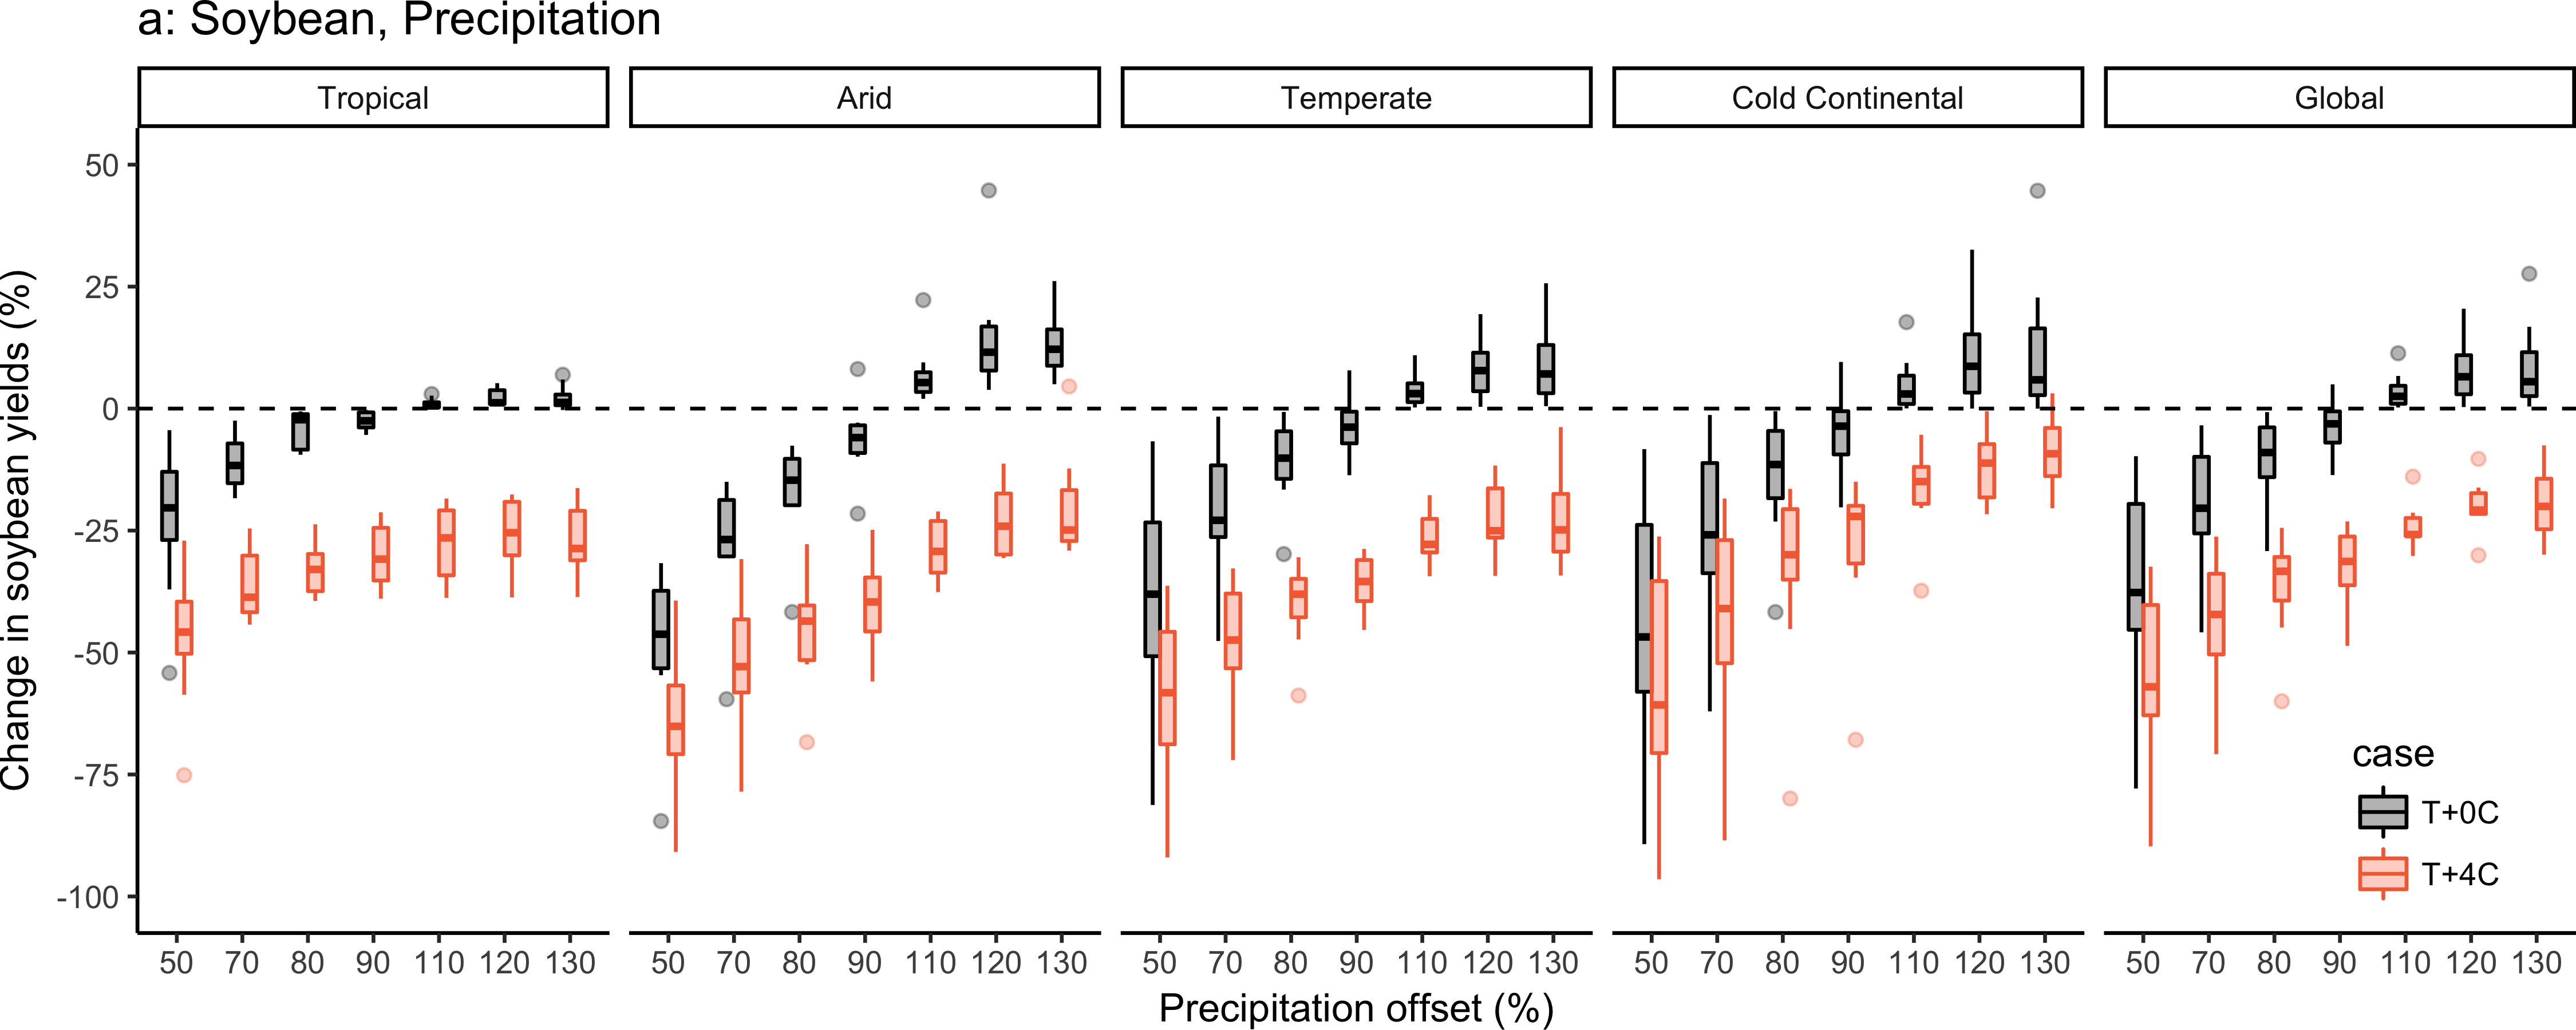
\includegraphics[width=15cm]{figures/soy_sim_CG_W.png}
   \caption{Illustration of the distribution of regional yield changes across the multi-model ensemble, split by K\"{o}ppen-Geiger climate regions for soy. Same as Figure \ref{fig:globesim} except precipitation is varied. Simulations at a T + 4K are show in color. Cold continental and polar regions are not shown because very little irrigated rice is grown in these regions.}
   \label{fig:globesim_W}
\end{figure*}

\begin{figure*}[ht]
\centering
   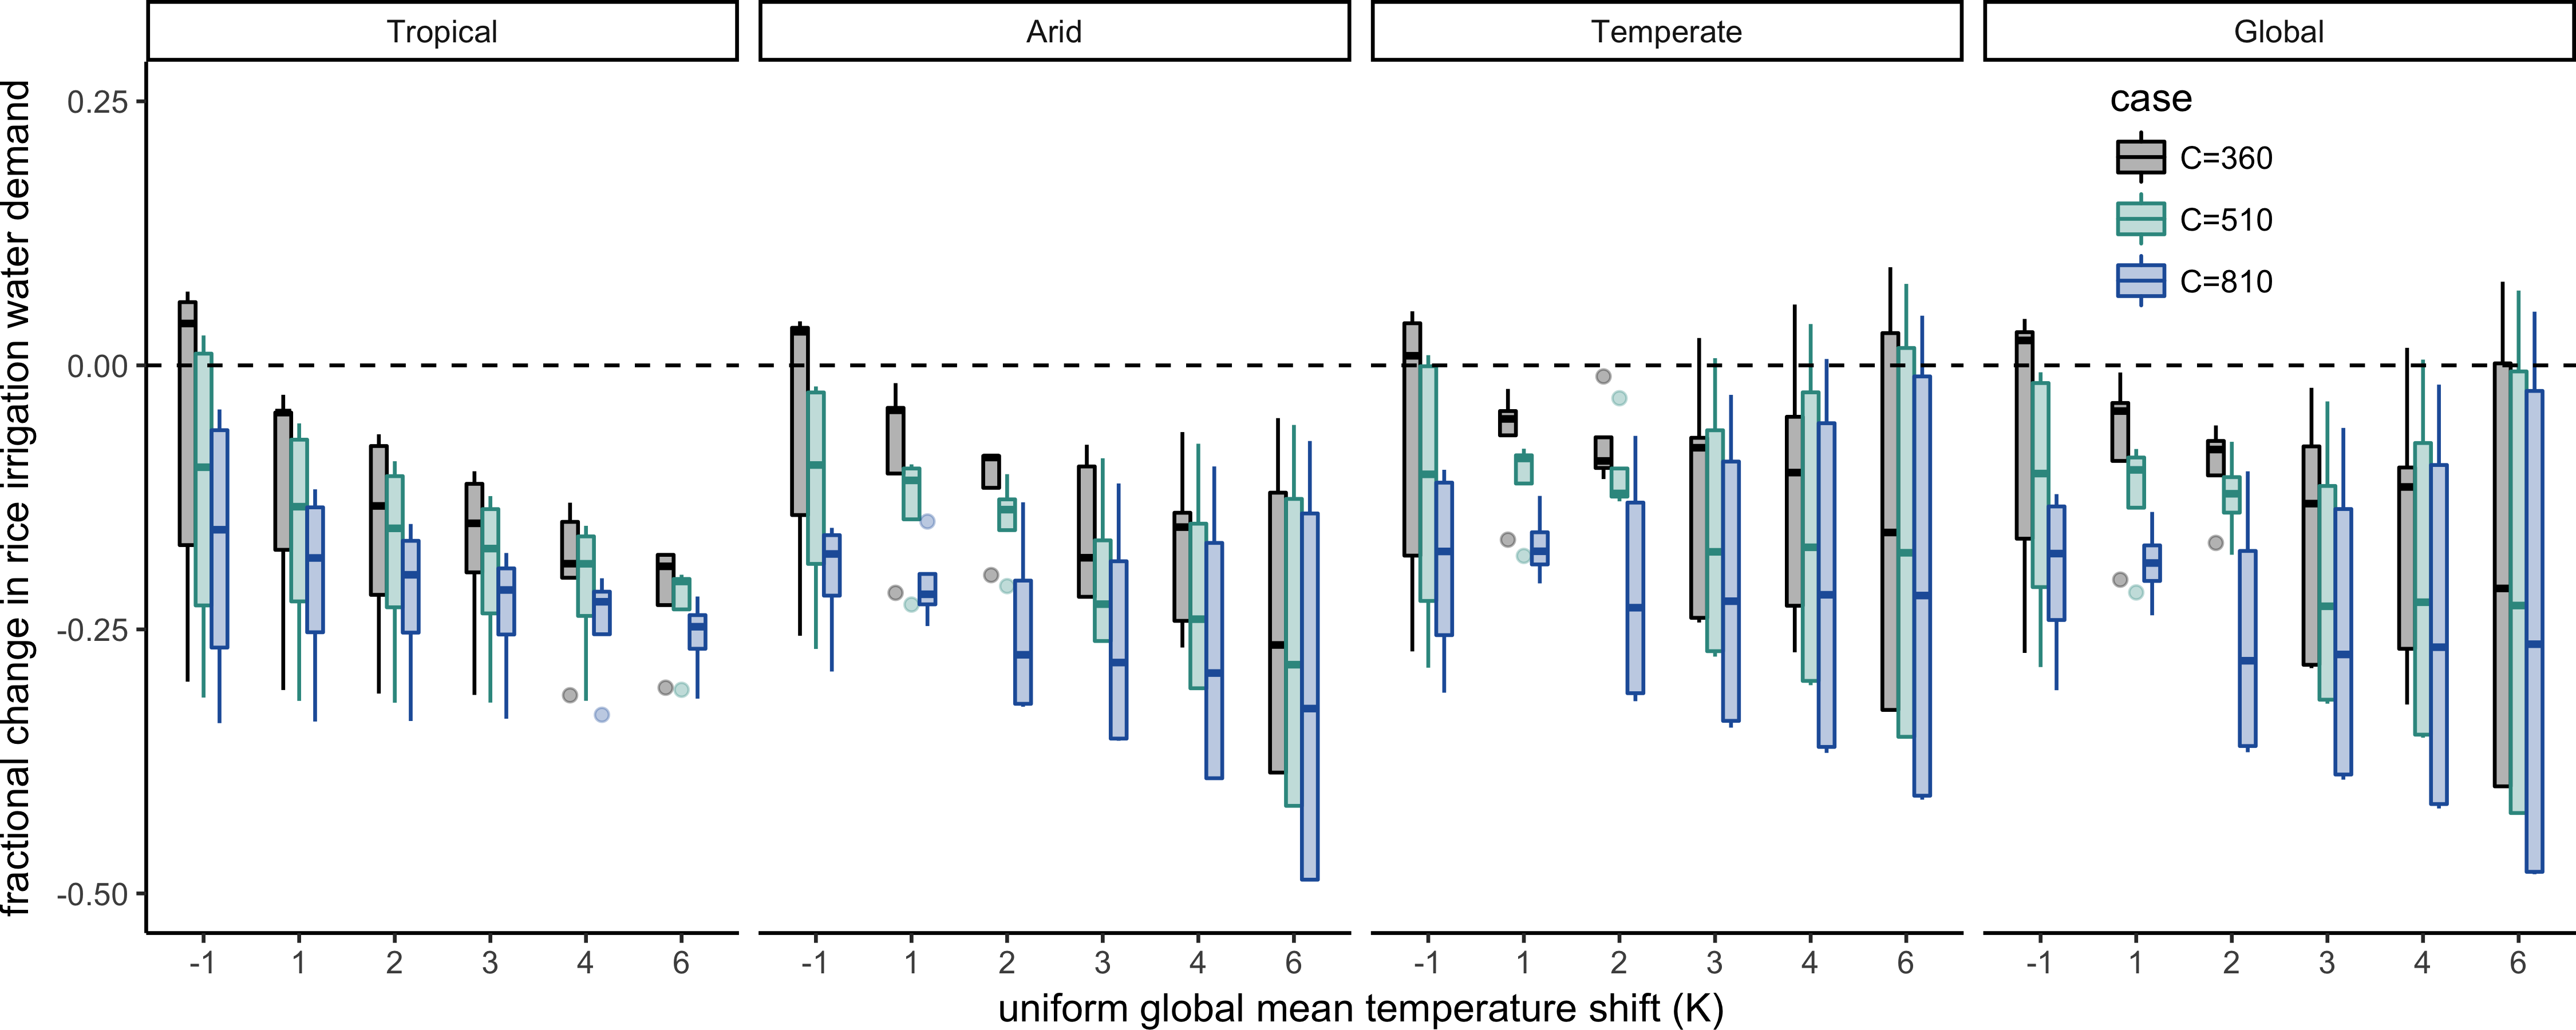
\includegraphics[width=14cm]{figures/rice_sim_CG_irrwat.png}
   \caption{Illustration of the distribution of regional irrigation water demand across the multi-model ensemble, split by K\"{o}ppen-Geiger climate regions for rice.}
   \label{fig:globesim_IRR}
\end{figure*}

Crop models in the GGCMI Phase II ensemble show broadly consistent responses to climate and management perturbations in most regions, with a strong negative impact of increased temperature in all but the coldest regions. 
Mapping the distribution of baseline yields and yield changes shows the geographic dependencies that underlie these results. Crop cultivation areas and yield changes with respect to the T+4 scenario show distinct geographic pattern (Figure \ref{fig:maizesoybaseline}). 
Absolute yield potentials show strong spatial variation, with much of the Earth's surface area unsuitable for any of these crops. 
In general, models agree most on yield response in regions where yield potentials are currently high and therefore where crops are currently grown. 
Models show robust decreases in yields at low latitudes, and highly uncertain median increases at most high latitudes, due in part to how crop failures are considered across different models. 
For wheat crops see Figure S16 wheat projections are more uncertain, possibly because simulation calibration is especially important \citep[e.g.][]{Asseng2013}.

We illustrate the across-model spread for rainfed maize in Figure \ref{fig:globesim}, which shows yields across all grid cells for the primary K\"{o}ppen-Geiger climate regions \citep{rubel2010}. 
In warming scenarios with precipitation held constant, all models show decreases in maize yield in the `warm temperate', `equatorial', and `arid' regions that account for nearly three-quarters of global maize production. 
These impacts are robust for even moderate climate perturbations. 
In the `warm temperate' zone, even a 1 degree temperature rise with other variables held fixed leads to a median yield reduction that exceeds the variance across models. 
A 6 degree temperature rise results in median loss of $\sim$25\% of yields with a signal to noise ratio of nearly three to one. A notable exception is the `cold continental' region, where models disagree strongly, extending even to the sign of impacts. 
Other crops show similar responses to warming, with robust yield losses in warmer locations and high inter-model variance in the `cold continental' regions (Figure S5).

The effects of rainfall changes on maize yields shown in Figure \ref{fig:globesim} are also as expected and are consistent across models. 
Increased rainfall mitigates the negative effect of higher temperatures by counteracting the increased evapo-transpiration to some degree, most strongly in arid regions.
Decreased rainfall amplifies yield losses and also increases inter-model variance; i.e. models agree that the response to decreased water availability is negative in sign but disagree on its magnitude.
%Decreased rainfall amplifies yield losses and also increases inter-model variance more strongly, suggesting that models have difficulty representing crop response to water stress or increased evapo-transpiration due to warmer temperatures. 
We show only rainfed maize here; see Figure S6 for comparison between rainfed and irrigated case. As expected, irrigated crops are more resilient to temperature increases in all regions, especially so where water is limiting. See Figures S7-15 in the supplement for other crops.   


\begin{figure}[ht]
\centering
   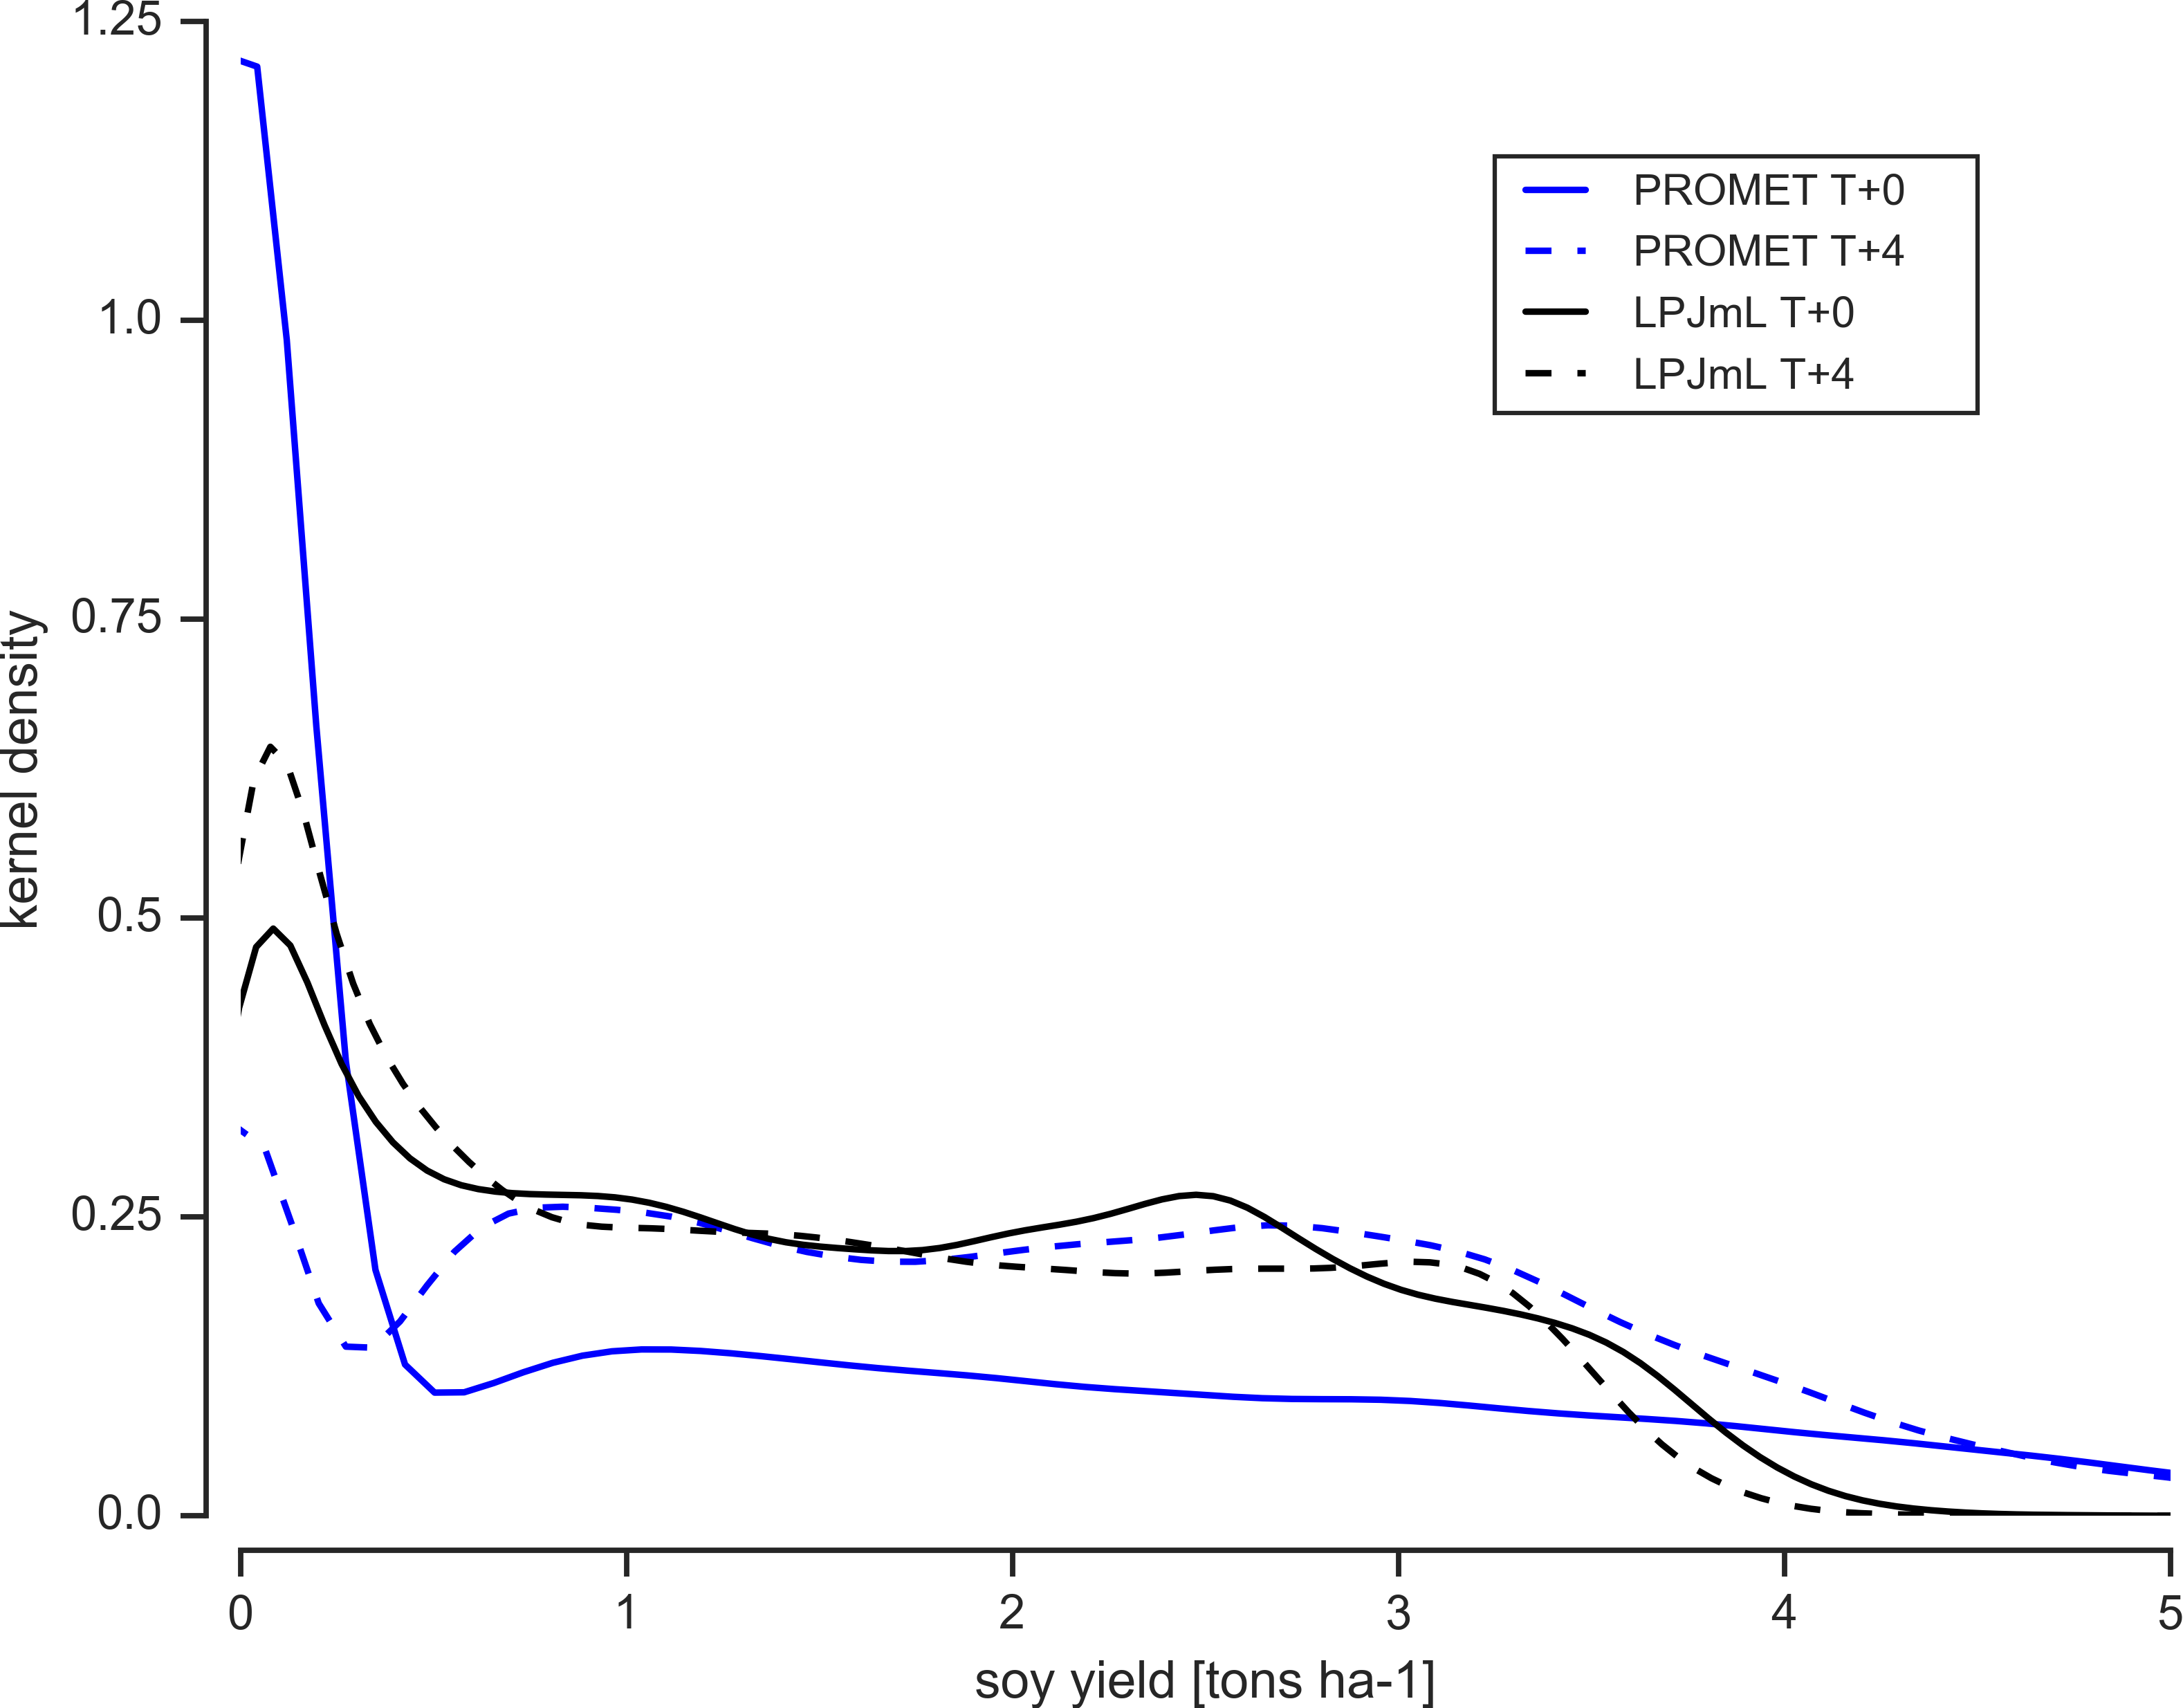
\includegraphics[width=8.3cm]{figures/testhighlatskde.png}
\caption{Kernel density estimate of soy yields north of 45$^o$ latitude for the PROMET and LPJmL models. Solid lines show the historical climatology and dashed lines show the T+4 (K) case. Note strong reduction in the lowest bin for the T+4 case for PROMET that is spread almost equally over the rest of the distribution.}
\label{fig:highlat}
\end{figure}

\section{Discussion and Conclusions} 
\label{S:5}
The GGCMI Phase II experiment provides a database designed to allow detailed study of crop yields from process-based models under climate change. 
The use of systematic input parameter variations facilitates not only comparing the sensitivities of process-based crop yield models to changing climate and management inputs but also evaluating the complex interactions between driving factors (CO$_2$,, temperature, precipitation, and applied nitrogen). 
Its global extent also allows identifying geographic shifts in high yield potential locations. 
We expect that the simulations will yield multiple insights in future studies, and show a selection of preliminary results. We discuss below implications from XXX

First, the GGCMI Phase II simulations allow identifying major areas of uncertainty. 
Inter-model uncertainty is qualitatively similar across all four inputs tested at the globally aggregate level with some notable exceptions. 
For example, soy, a nitrogen-fixing legume, is insensitive to nitrogen addition, while wheat is particularly uncertain in its response to CO$_2$, levels and water availability (Figure S22). 
Across geographic regions, projections are most robust in the low latitudes where yield impacts are largest, and most uncertain in the high latitudes where yields may increase. 
Model differences in projected high-latitude yield changes appear driven more by differences in baseline than in future yields.  
PROMET, for example, involves a stronger response to cold than does LPJmL, with frost below -8 °C irreversibly killing non-winter crops and prolonged periods of below-optimum temperatures also leading to complete crop failure. 
Over the high-latitudes regions simulated by both models, 52\% of grid cells in PROMET report 0 yield in the present climate vs. 11\% of cells in the T+4 scenario, leading to a strong yield gain in warmer future climates. 
In LPJmL, the same high-latitude area is suitable for cultivation even in baseline climate, with crop failure rates of 4\% and 5\% in present and T+4 cases, so that projected yield changes are modest (Figure S23.)

Second, the GGCMI Phase II simulations demonstrate the sensitivity of climate-driven yield impacts to the locations of cultivated land. 
One counterintuitive result apparent in the simulations is that warmer temperatures drive steeper yield reductions in irrigated than rainfed maize when considered only over currently cultivated land, even though water availability increases crop resiliency to temperature increases at any given location (compare Figure \ref{fig:globe_em} to Figure \ref{fig:globesim} and Figures S6 to S7). 
The effect results from geographic differences in cultivation: irrigated maize is grown in warmer locations where the impacts of warming are more severe. 
(See Figures S8-S15 for other crops.) 
Geographic effects also mean that nitrogen fertilization produces stronger responses in irrigated than non-irrigated wheat and maize, presumably because those rainfed crops are limited by water availability (Figure S21).

In general, the development of multi-model ensembles involving systematic parameters sweeps has large promise for increasing understanding of potential future crop responses and for improving process-based crop models.

%%%%%%%%%%%%%%%%%%%%%%%%%%%%%%%%%%%%%%%%%%%%%%%%%%%%%%%%%%%%%%%
\codedataavailability{The simulation outputs of the mandatory 7 output variables (Table \ref{table:outputs}) are available on zenodo.org. 
See Appendix \ref{A:1} for data DOIs. 
All other simulation output variables are available upon request to the corresponding author. The scripts for generating the spring wheat and winter wheat growing seasons and second fertilizer dates and the quality screening script is available at https://github.com/RDCEP/ggcmi/blob/phase2/.
All input data are available via globus.org (registration required, free of charge):
Minimum cropland mask is available at
\url{https://www.globus.org/app/transfer?origin\_id=e4c16e81-6d04-11e5-ba46-22000b92c6ec&origin\_path=\%2FAgMIP.input\%2FCTWN\%2F}
choose the file boolean\_cropmask\_ggcmi\_phase2.nc4
Growing period data for wheat is now divided up into winter and spring wheat, available at
\url{https://www.globus.org/app/transfer?origin\_id=e4c16e81-6d04-11e5-ba46-22000b92c6ec&origin\_path=\%2FAgMIP.input\%2Fother.inputs\%2FAGMIP\_GROWING\_SEASON.HARM.version2.0\%2F}
whereas all other growing season data (maize, rice, soybean) are the same as in phase 1 (version 1.25), available at
\url{https://www.globus.org/app/transfer?origin\_id=e4c16e81-6d04-11e5-ba46-22000b92c6ec&origin_path=\%2FAgMIP.input\%2Fother.inputs\%2FAGMIP\_GROWING\_SEASON.HARM.version1.25\%2F}
}

\appendix
\section{}
\subsection{Data Access}
\label{A:1}
Simulation yield output dataset can be found at the DOIs located in table \ref{table:dataloc}.

\begin{table*}[t]
\caption{DOI's for model yield data outputs. All yield output data can be found at https://doi.org/10.5281/zenodo/XX. Where XX is the value found in the table.} 
\label{table:dataloc}
	\begin{tabular}{p{3cm} p{1.5cm} p{1.5cm} p{1.5cm} p{1.5cm} p{1.5cm}}
        \tophline
        {\textbf{Model}}&{\textbf{Maize}}&{\textbf{Soy}}&{\textbf{Rice}}&{\textbf{Winter wheat}}&{\textbf{Spring wheat}}\\ \middlehline
        {\textbf{APSIM-UGOE}} & {2582531} & {258235} & {2582533} & {2582537} & {2582539}\\ \middlehline
        {\textbf{CARAIB}} & {2582522} & {2582508} & {2582504} & {2582516} & {2582499}\\ \middlehline
        {\textbf{EPIC-IIASA}} & {2582453} & {2582461} & {2582457} & {2582463} & {2582465}\\  \middlehline
        {\textbf{EPIC-TAMU}} & {2582349} & {2582367} & {2582352} & {2582392} & {2582418}\\ \middlehline
        {\textbf{JULES}} & {2582543} & {2582547} & {2582545} & {--} & {2582551}\\ \middlehline
        {\textbf{GEPIC}} & {2582247} & {258225} & {2582251} & {2582260} & {2582263}\\ \middlehline
        {\textbf{LPJ-GUESS}} & {2581625} & {--} & {--} & {2581638} & {2581640}\\  \middlehline
        {\textbf{LPJmL}} & {2581356} & {2581498} & {2581436} & {2581565} & {2581606}\\ \middlehline
        {\textbf{ORCHIDEE-crop}} & {2582441} & {--} & {2582445} & {2582449} & {--}\\ \middlehline
        {\textbf{pDSSAT}} & {2582111} & {2582147} & {2582127} & {2582163} & {2582178}\\ \middlehline
        {\textbf{PEPIC}} & {2582341} & {2582433} & {2582343} & {2582439} & {2582455}\\ \middlehline
        {\textbf{PROMET}} & {2582467} & {2582488} & {2582479} & {2582490} & {2582492}\\
        \bottomhline
    \end{tabular}
\end{table*}
\noappendix %% use this to mark the end of the appendix section

\authorcontribution{J.E., C.M, A.R., J.F., and E.M.\ designed the research. C.M., J.J., J.B., P.C., M.D., P.F., C.F., L.F., M.H., C.I., I.J., C.J., N.K., M.K., W.L., S.O., M.P., T.P., A.R., X.W., K.W., and F.Z.\ performed the simulations. J.F., J.J., A.S., M.L., and E.M.\ performed the analysis and J.F. and E.M.\ prepared the manuscript.}

\competinginterests{The authors declare no competing interests.}

\begin{acknowledgements}
This research was performed as part of the Center for Robust Decision-Making on Climate and Energy Policy (RDCEP) at the University of Chicago, and was supported through a variety of sources. 
RDCEP is funded by NSF grant \#SES-1463644 through the Decision Making Under Uncertainty program. 
J.F.\ was supported by the NSF NRT program, grant \#DGE-1735359. 
C.M.\ was supported by the MACMIT project (01LN1317A) funded through the German Federal Ministry of Education and Research (BMBF). 
C.F.\ was supported by the European Research Council Synergy grant \#ERC-2013-SynG-610028 Imbalance-P. 
P.F.\ and K.W.\ were supported  by the Newton Fund through the Met Office Climate Science for Service Partnership Brazil (CSSP Brazil). 
K.W.\ was supported by the IMPREX research project supported by the European Commission under the Horizon 2020 Framework programme, grant \#641811. 
A.S.\ was supported by the Office of Science of the U.S. Department of Energy as part of the Multi-sector Dynamics Research Program Area. 
S.O.\ acknowledges support from the Swedish strong research areas BECC and MERGE together with support from LUCCI (Lund University Centre for studies of Carbon Cycle and Climate Interactions). 
R.C.I.\ acknowledges support from the Texas Agrilife Research and 634 Extension, Texas A \&M University. This is paper number 35 of the Birmingham Institute of Forest Research. Computing resources were provided by the University of Chicago Research Computing Center (RCC).
\end{acknowledgements}

%% Since the Copernicus LaTeX package includes the BibTeX style file copernicus.bst,
\bibliographystyle{copernicus}
\bibliography{bib}

\end{document}